\documentclass[12pt]{aghdpl}
% \documentclass[language=en,11pt]{aghdpl}  % praca w języku angielskim

%---------------------------------------------------------------------------

\author{Tristan Malatyński}
\shortauthor{Tristan Malatyński}

\titlePL{Implementacja gry muzycznej z wykorzystaniem instrumentu klawiszowego i analizy sygnałów dźwiękowych
}

\titleEN{Implementation of a music game using a keyboard instrument and sound signal analysis}


\shorttitlePL{Implementacja gry muzycznej z wykorzystaniem analizy sygnałów dźwiękowych} % skrócona wersja tytułu jeśli jest bardzo długi
\shorttitleEN{}
\usepackage{float}
% Dopuszczalne wartości[1,2]:
% * "Projekt dyplomowy" - na koniec studiów I stopnia
% * "Praca dyplomowa" - na koniec studiów II stopnia
% [1] Zasady dyplomowania w roku akademickim 2020/2021 (Decyzja Dziekana WEAIiIB nr 16/2020 z dnia 9 grudnia 2020 roku)
% [2] Załącznik nr 1a) do Decyzji nr 16/2020 Dziekana Wydziału EAIiIB z dnia 09 grudnia 2020 r.
\thesistype{Projekt dyplomowy}
%\thesistype{Master of Science Thesis}

\supervisor{dr inż. Piotr Pawlik}
%\supervisor{Paweł Kłeczek, PhD}

\degreeprogramme{Automatyka i Robotyka}
%\degreeprogramme{Automatics and Robotics}

\date{2024}

%\department{Katedra Informatyki Stosowanej}
%\department{Department of Applied Computer Science}

\faculty{Wydział Elektrotechniki, Automatyki, Informatyki i Inżynierii Biomedycznej}
%\faculty{Faculty of Electrical Engineering, Automatics, Computer Science and Biomedical Engineering}

\acknowledgements{Dedykuję tę pracę wszystkim, którzy byli ze mną w chwilach radości i którzy nie pozwolili upaść w chwilach strapienia}


\begin{document}


	\titlepages
	\RedefinePlainStyle
	
	\setcounter{tocdepth}{2}
	\tableofcontents
	\clearpage
        \chapter{Wstęp}
\vspace{-30pt}
\section{Wprowadzenie do tematu }
Chcąc nauczyć się grać utwór muzyczny na instrumencie klawiszowym, najpierw trzeba nabyć umiejętność czytania nut oraz znaleźć zapis nutowy danej piosenki. Można również wyświetlić piosenkę w postaci graficznie przedstawionych wskazówek, które klawisze należy naciskać i jak długo (tzw. synthesii), aby zagrać dany utwór, niemniej jednak wymaga to od nas znalezienia gotowej animacji, bądź piosenki w formacie muzycznym midi, który rzadko występuje oraz program, który ten format przekonwertuje i wyświetli. Dużo łatwiej uzyskać plik muzyczny wav lub mp3. Dzięki postępom w dziedzinie analizy sygnałów audio możliwe stało się mapowanie dźwięków z plików mp3 na sekwencje nut w formacie midi. Ten proces konwersji, wykorzystujący zaawansowane techniki przetwarzania sygnałów, otwiera drzwi do nowych metod edukacyjnych, umożliwiając naukę gry na instrumentach muzycznych w interaktywny i atrakcyjny sposób.
\section{Cel pracy inżynierskiej}
Głównym celem niniejszej pracy inżynierskiej jest stworzenie programu w postaci gry muzycznej zintegrowanej z elektronicznym instrumentem klawiszowym, gdzie następuje przedstawienie w postaci graficznej wyznaczonych uprzednio tonów i porównywanie do sygnału odbieranego z keyboardu oraz naliczanie punktów za poprawne odwzorowywanie sekwencji klawiszy.
Dodatkowym wyzwaniem jest również opracowanie sposobu konwersji plików muzycznych z formatu mp3 do formatu midi poprzez przeanalizowanie sygnału audio z wykorzystaniem transformaty Fouriera i analityczne wyznaczenie częstotliwości z powstałego widma.
\newpage
\section{Struktura i zakres pracy}
W dalszej części pracy zostały szczegółowo omówione teoretyczne podstawy syntezy dźwięku oraz analizy sygnałów audio. Następnie została przedstawiona metodyka obejmująca proces konwersji plików mp3 do formatu midi. Kolejny rozdział zawiera szczegółowy opis implementacji gry umożliwiającej wizualizację wygenerowanej synthesii interaktywnej z keyboardem użytkownika, co pozwala na uzyskiwanie punktów za poprawne powtarzanie wyświetlonej sekwencji klawiszy.

\begin{figure}[h]
  \centering
  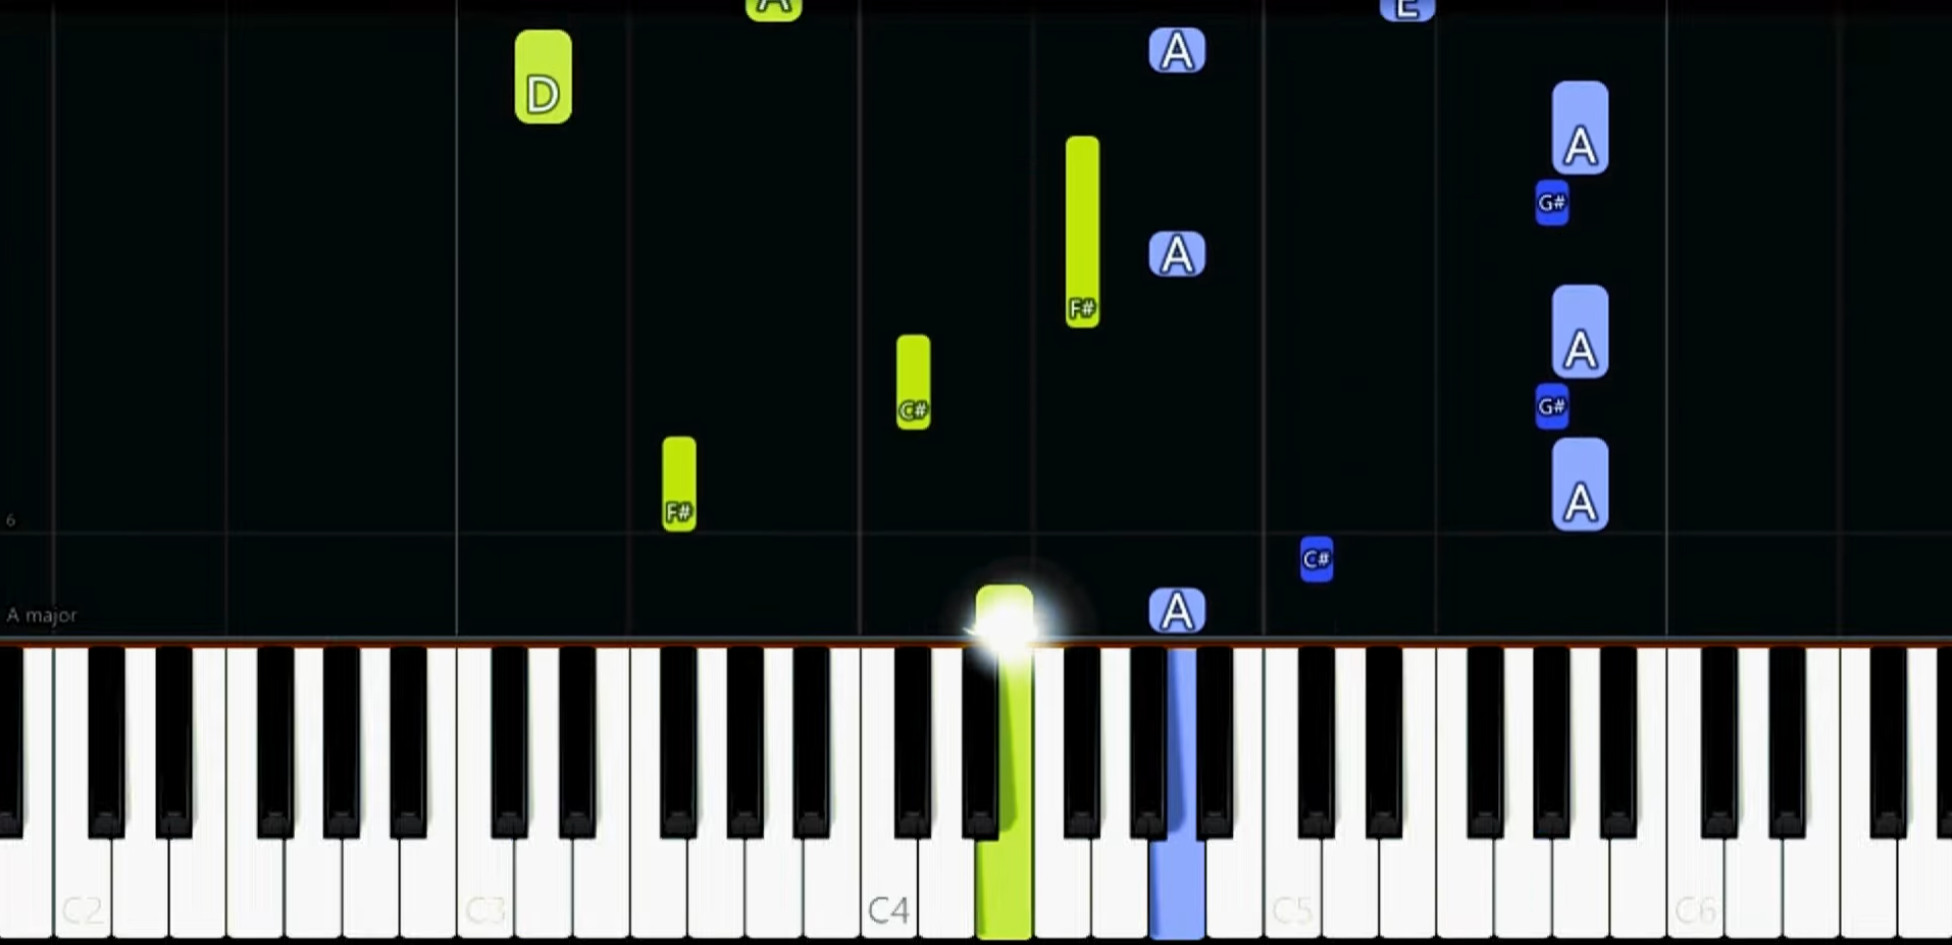
\includegraphics[width=1\textwidth]{img/1/image.png}
  \caption{Przykładowa synthesia przedstawiająca piosenkę Yiruma - "River Flows In You"\cite{synthesia}}
\end{figure}

Dalsza część pracy poświęcona będzie testowaniu projektu i analizie uzyskanych wyników, rozważań nad osiągniętymi rezultatami oraz perspektywom rozwoju projektu w kontekście możliwych usprawnień i dalszych badań. Niniejsza praca stanowi wkład w rozwój technologii przetwarzania sygnałów audio oraz otwiera nowe możliwości w zakresie interaktywnej edukacji muzycznej i kreatywnej ekspresji dźwiękowej. Eksploracja tych zaawansowanych technik konwersji dźwięku ma na celu stworzenie narzędzia, które może znaleźć zastosowanie w edukacji oraz rozrywce.
\newpage
\section{Wykorzystane narzędzia}

Implementacja gry muzycznej z użyciem instrumentu klawiszowego wymaga bardzo elastycznego i nieograniczającego środowiska oraz wielu narzędzi, które zapewnią wiele możliwości na jakże obszernym polu, które obejmuje projekt. Środowisku, które sprawdzi się w analizie sygnałów dźwiękowych, pozwalające również na przetwarzanie dużej ilości danych w krótkim czasie, aby program był użytkowy. Idealnie do powyższej problematyki wpasowuje się język programowania {Python} \cite{python}, często wybierany w projektach związanych z przetwarzaniem wszelakich sygnałów ze względu na elastyczność, prostotę i bogactwo w dostępności bibliotek pomocnych w obliczeniach takich jak {NumPy} \cite{numpy}, do pracy z dźwiękiem jak przykładowo {LibROSA} \cite{librosa}, czy do wizualizacji danych takich jak {Matplotlib} \cite{matplotlib}.

Bardzo ważnym elementem jest biblioteka {Pygame} \cite{pygame}, która pomaga nie tylko w tworzeniu projektu w postaci gry, ale również sprawdza się jako pomoc przy znalezieniu podłączonego instrumentu muzycznego i odebraniu z niego danych. Zazwyczaj komputery osobiste nie posiadają wejścia MIDI, ale użycie interfejsu audio MIDI USB \cite{roland_um_one} marki Roland pozwala przetworzyć sygnał pochodzący z instrumentów, takich jak np. keyboard CASIO \cite{casio_ctk496}.

Jednak aby można było wykorzystać instrument w testowaniu projektu, niezbędna jest możliwość przetworzenia sygnału midi na plik muzyczny oraz manipulowania nim w kolejnych etapach, w czym nieocenione były narzędzia {FluidSynth} \cite{fluidsynth} oraz {FFmpeg} \cite{ffmpeg} dające szerokie spektrum możliwości.

Aby dokładnie przeprowadzić analizę sygnału ścieżki audio niezbędnym narzędziem jest transformata Fouriera \cite{fourier_transform_visual}\cite{dsp_understanding}, która pozwala spojrzeć na ten sam sygnał w całkowicie inny sposób.

Ostatnią czynnością pozostało zamknięcie wszystkich elementów w jedną całość, zachowując pełną funkcjonalność, jednakże nie odstając szatą graficzną. Pozwoliło na to użycie {pygame-menu} \cite{pygame_menu} oraz {Tkinter} \cite{tkinter} dzięki czemu gotowy program nie tylko jest efektywny, ale również efektowny.

        \chapter{Podstawy teoretyczne}
\vspace{-25pt}
\section{Omówienie teorii sygnałów dźwiękowych}
\subsection{Główne elementy dźwięku}

\textbf{Częstotliwość} odpowiada za wysokość tonu, więc manipulowanie częstotliwością, pozwala na uzyskanie całej gamy melodycznej, a zatem zróżnicowanego brzmienia utworów. Częstotliwość to ilość cykli fali dźwiękowej występujących w jednostce czasu. Podawana w hertzach, gdzie jeden Hz oznacza jeden cykl na sekundę. Dla ludzkiego ucha zakres częstotliwości słyszalnych wynosi zazwyczaj od około 20 Hz do 20 000 Hz (20 kHz). Każdy ton ma ustaloną odpowiednią częstotliwość. Częstotliwość tego samego tonu o oktawę wyższego jest dwukrotnie większa

\begin{table}[H]
\centering
\caption{Częstotliwości tonów zaokrąglone do 2 po przecinku \cite{piano_key_frequencies}}
\label{tab:frequency}
\begin{tabular}{@{}lrrrrrrrrr@{}}
\toprule
Ton/Oktawa & 0    & 1    & 2     & 3      & 4       & 5       & 6        & 7        & 8        \\ \midrule
C          & 16.35 & 32.7 & 65.41 & 130.81 & 261.63 & 523.25 & 1046.5 & 2093 & 4186 \\
C\#        & 17.32 & 34.65 & 69.3 & 138.59 & 277.18 & 554.37 & 1108.73 & 2217.46 & 4434.92 \\
D          & 18.35 & 36.71 & 73.42 & 146.83 & 293.66 & 587.33 & 1174.66 & 2349.32 & 4698.63 \\
D\#        & 19.45 & 38.89 & 77.78 & 155.56 & 311.13 & 622.25 & 1244.51 & 2489 & 4978 \\
E          & 20.06 & 41.2 & 82.41 & 164.81 & 329.63 & 659.25 & 1318.51 & 2637 & 5274 \\
F          & 21.83 & 43.65 & 87.31 & 174.61 & 349.23 & 698.46 & 1396.91 & 2793.83 & 5587.65 \\
F\#        & 23.12 & 46.25 & 92.5 & 185 & 369.99 & 739.99 & 1479.98 & 2959.96 & 5919.91 \\
G          & 24.05 & 49 & 98 & 196 & 392 & 783.99 & 1567.98 & 3135.96 & 6271.93 \\
G\#        & 25.96 & 51.91 & 103.83 & 207.65 & 415.3 & 830.61 & 1661.22 & 3322.44 & 6644.88 \\
A          & 27.05 & 55 & 110 & 220 & 440 & 880 & 1760 & 3520 & 7040 \\
A\#        & 29.14 & 58.27 & 116.54 & 233.08 & 466.16 & 932.33 & 1864.66 & 3729.31 & 7458.62 \\
B          & 30.87 & 61.74 & 123.47 & 246.94 & 493.88 & 987.77 & 1975.53 & 3951 & 7902.13 \\ \bottomrule
\end{tabular}
\end{table}

\textbf{Amplituda} odnosi się do głośności dźwięku. Oznacza to odchylenie wartości dźwięku od stanu spoczynkowego, czyli jak mocno drgają cząsteczki medium (np. powietrza). Mierzona w decybelach, co odnosi się do logarytmicznej skali, gdzie każda zwiększona liczba dB oznacza podwojenie siły dźwięku.

\textbf{Barwa dźwięku} zwana także timbre, odnosi się do charakterystycznej jakości dźwięku, która pozwala odróżnić dźwięki o tej samej wysokości i głośności, ale pochodzące od różnych instrumentów lub źródeł. Zależna od składowych harmonicznych, czyli częstotliwości składników wibracyjnych w dźwięku. Różnice w ilości i intensywności składowych harmonicznych powodują, że te same tony zagrane na różnych instrumentach mają kompletnie różne brzmienie.

\subsection{Synteza dźwięku}

Synteza dźwięku \cite{sound_synthesis} to proces generowania dźwięku, który może być wykonywany na wiele różnych sposobów, zależnie od celu, rodzaju dźwięku i kreatywnych intencji. Ogólnie rzecz biorąc, synteza dźwięku polega na tworzeniu dźwięków od podstaw lub na ich modyfikowaniu, aby osiągnąć pożądane brzmienie. Oto kilka kluczowych aspektów syntezy dźwięku:\\

\noindent\textbf{Generowanie dźwięku}

Synteza może polegać na tworzeniu dźwięku od podstaw przy użyciu oscylatorów, generujących fale dźwiękowe o określonych częstotliwościach i kształtach. Może też opierać się na wykorzystaniu zapisanych dźwięków (próbek) jako źródła generowania dźwięku.\\

\noindent\textbf{Manipulacja parametrami}

Synteza umożliwia modyfikowanie parametrów dźwięku, takich jak wysokość tonu, głośność, kształt fali dźwiękowej, czas trwania czy charakterystyka przestrzenna (panoramowanie). Możliwość kontrolowania tych parametrów pozwala na kształtowanie brzmień i tworzenie różnorodnych dźwięków.\\

\noindent\textbf{Tworzenie różnorodnych brzmień}

Dzięki różnym technikom syntezy możliwe jest generowanie różnorodnych brzmień, od prostych tonów po złożone struktury dźwiękowe. Niektóre metody syntezy pozwalają na realistyczne emulacje instrumentów muzycznych, podczas gdy inne skupiają się na tworzeniu bardziej abstrakcyjnych i eksperymentalnych dźwięków.\\

\noindent\textbf{Wykorzystanie w produkcji muzycznej}

Synteza dźwięku jest szeroko stosowana w produkcji muzycznej, w syntezatorach, samplerach, programach do tworzenia muzyki elektronicznej oraz w aplikacjach do postprodukcji dźwięku. Oparta jest na manipulacji parametrów dźwięku lub wykorzystaniu istniejących dźwięków do tworzenia nowych brzmień, co daje twórcom szerokie możliwości eksperymentowania i kreowania unikalnych dźwięków.\\

\noindent\textbf{Rodzaje syntez}

• Synteza Subtraktywna:
Metoda oparta na filtracji i modelowaniu harmonicznych elementów dźwięku.
Generuje dźwięk poprzez usuwanie (subtrakcję) części harmonicznych z bogatszego sygnału źródłowego.\\

• Synteza Addytywna:
Generowanie dźwięku przez sumowanie wielu prostych fal sinusoidalnych o różnych częstotliwościach i amplitudach.
Tworzone brzmienia są bardziej złożone ze względu na dodawanie wielu harmonicznych składowych.\\


• Synteza FM (Frequency Modulation):
Technika syntezy, w której jedna fala moduluje częstotliwość kolejnej fali harmonicznej, co generuje barwne i bogate brzmienie.
Oparta na zmianie częstotliwości nośnej poprzez sygnał modulatora.\\


• Synteza Granularna:
Opiera się na manipulacji i kombinowaniu mikroskopijnych fragmentów dźwięku zwanych ziarnami.
Dźwięk jest generowany poprzez sekwencyjne odtwarzanie, modyfikację i łączenie krótkich fragmentów dźwiękowych.\\

• Synteza Wavetable:
Wykorzystuje gotowe cyfrowe tabelki (wavetable) jako źródło dźwięku.
Generuje dźwięk poprzez odtwarzanie cyfrowych próbek dźwięku zapisanych w tabelach.\\


• Synteza Fizyczna (Physical Modeling):
Symuluje zachowanie fizycznych instrumentów muzycznych przez matematyczne modele ich akustyki.
Generuje dźwięk, opierając się na równaniach, które opisują zachowanie instrumentów.\\



• Synteza Formantowa:
Opiera się na modelowaniu rezonansowych częstotliwości w ludzkim aparacie głosowym.
Generuje dźwięk poprzez manipulację rezonansami, imitując brzmienie mowy i ludzkiego głosu.\\

• Synteza Próbkowa:
Wykorzystuje gotowe cyfrowe próbki dźwiękowe jako podstawę generowania dźwięku.
Odtwarza zapisane dźwięki instrumentów lub innych źródeł, umożliwiając manipulację parametrów dźwięku.\\

	Każda z powyższych technik syntezy dźwięku oferuje unikalne możliwości generowania różnorodnych brzmień i znalazła zastosowanie w różnych obszarach produkcji muzycznej, eksperymentalnej oraz w inżynierii dźwięku.


\section{Transformata Fouriera}

Transformata Fouriera jest narzędziem matematycznym, które umożliwia analizę funkcji czasowej poprzez jej dekompozycję na składowe częstotliwościowe. To narzędzie, które pozwala spojrzeć na sygnał z innej perspektywy, przenosząc go z dziedziny czasu (przestrzeń czasowo-amplitudowa) na dziedzinę częstotliwości (przestrzeń częstotliwościowo-amplitudowa) \cite{fourier_transform_visual}\cite{dsp_understanding}.

\begin{equation}
F(\omega) = \int_{-\infty}^{\infty} -f(t) e^{-j\omega t} \,dt
\end{equation}
gdzie:
\begin{itemize}
    \item \(F(\omega)\) jest transformacją Fouriera funkcji \(f(t)\),
    \item \(\omega\) jest częstotliwością kątową,
    \item \(j\) jest jednostką urojoną.
\end{itemize}

Transformata Fouriera posiada wiele ważnych właściwości, które czynią ją niezwykle użyteczną w analizie sygnałów. Niektóre z tych właściwości to:
Liniowość: Transformata Fouriera jest liniowa, co oznacza, że transformata sumy dwóch sygnałów jest równa sumie transformacji tych sygnałów.
Przesunięcie czasowe: Przesunięcie sygnału w czasie powoduje zmianę fazy jego transformaty Fouriera, ale nie wpływa na jego amplitudę.
Przeskalowanie czasowe: Przeskalowanie sygnału w czasie powoduje odwrotne przeskalowanie w dziedzinie częstotliwości.
Dualność: Transformata Fouriera samej transformaty Fouriera sygnału daje sygnał zbliżony do oryginalnego odwróconego w czasie.
Transformata Fouriera jest niezwykle użyteczna w analizie sygnałów, ponieważ pozwala na rozłożenie złożonego sygnału na prostsze składniki, które są łatwiejsze do analizy. Na przykład, sygnał muzyczny może być rozłożony na składniki harmoniczne, które odpowiadają różnym dźwiękom instrumentów muzycznych. Analiza Fouriera to niezastąpione narzędzie zarówno w badaniach naukowych, jak i praktycznych zastosowaniach w dziedzinie dźwięku i syntezy.
\newpage
\subsection{Szybka Transformata Fouriera - FFT}
Szybka Transformata Fouriera to algorytm o niskiej złożoności obliczeniowej, służący do obliczania dyskretnej transformaty Fouriera DFT dla sekwencji N punktów w czasie znacznie szybciej niż bezpośrednie obliczenie DFT. Dla sekwencji N punktów, DFT jest zdefiniowana jako:

\begin{equation}
F(n) = \sum_{k=0}^{N-1} f(k) e^{-j\frac{2\pi}{N}nk}
\end{equation}
gdzie:
\begin{itemize}
    \item \(F(n)\) jest \(n\)-tym punktem DTF sekwencji \(f(k)\),
    \item \(k\) jest indeksem punktu w sekwencji,
    \item \(j\) jest jednostką urojoną,
    \item \(N\) jest całkowitą liczbą punktów w sekwencji.
\end{itemize}

FFT redukuje liczbę obliczeń z \(O(N^2)\) do \(O(N \log N)\) wykorzystując symetrię i okresowość DFT, co jest znacznym ulepszeniem.
Najpopularniejszym algorytmem FFT jest algorytm Cooley-Tukey. Jest to algorytm typu “dziel i zwyciężaj”, który dzieli DFT o rozmiarze N na dwie DFT o rozmiarze N/2, co pozwala na znaczne zredukowanie liczby obliczeń. Algorytm ten jest najefektywniejszy, gdy N jest potęgą liczby 2. FFT znajduje zastosowanie w wielu dziedzinach, takich jak przetwarzanie sygnałów audio i wideo, analiza sejsmiczna, przetwarzanie obrazów, telekomunikacja oraz w naukach fizycznych i inżynierskich. Umożliwia szybką konwolucję, filtrację sygnałów, analizę widmową oraz przetwarzanie sygnałów w czasie rzeczywistym. FFT jest niezbędnym narzędziem w pracy inżynierskiej, umożliwiającym efektywne przetwarzanie sygnałów i analizę danych. Zrozumienie i zastosowanie FFT pozwala na znaczące przyspieszenie obliczeń i jest kluczowe w wielu nowoczesnych technologiach.

\subsection{STFT}

Użycie STFT (Short-Time Fourier Transform) polega na analizie sygnału dźwiękowego w krótkich oknach czasowych, co pozwala na badanie zmian widma częstotliwościowego sygnału w czasie. Sygnał dźwiękowy jest dzielony na krótkie fragmenty, zwane ramkami, które często nakładają się na siebie. Każda ramka jest analizowana niezależnie od pozostałych. Na każdej ramce czasowej stosuje się transformatę Fouriera, co przekształca sygnał z dziedziny czasu na dziedzinę częstotliwości dla tej konkretnej ramki. Dla każdej ramki otrzymywane jest widmo częstotliwościowe, pokazujące składowe częstotliwościowe sygnału w tym konkretnym fragmencie czasu. STFT umożliwia analizę ewolucji widma częstotliwościowego w funkcji czasu. Dzięki analizie kolejnych ram czasowych można śledzić zmiany częstotliwości w sygnale w zależności od czasu.\\

\textbf{Zastosowania STFT}

• Spektrogramy: STFT jest podstawą do tworzenia spektrogramów, czyli graficznych reprezentacji zmian widma częstotliwościowego w czasie.

• Analiza sygnału: Pozwala na identyfikację zmian w zawartości częstotliwościowej sygnału w różnych momentach czasowych.

• Transpozycja dźwięku: Umożliwia zmianę wysokości tonu w utworach muzycznych poprzez manipulację ramkami czasowymi.\\

STFT jest ważnym narzędziem w analizie sygnału dźwiękowego, pozwalającym na szczegółową analizę zmian widma częstotliwościowego w zależności od czasu, co ma zastosowanie w wielu dziedzinach, od analizy dźwięku po inżynierię dźwięku i przetwarzanie sygnałów.

\section{Formaty plików dźwiękowych}

\noindent\textbf{MP3 (MPEG-1 Audio Layer III)}

MP3 jest formatem kompresji stratnej, redukującym rozmiar pliku poprzez usuwanie danych nieistotnych dla ludzkiego ucha. Przechowuje dźwięk w formie skompresowanej, usuwając pewne elementy, co prowadzi do utraty niektórych detali audio. Powszechnie wykorzystywany do przechowywania muzyki w plikach cyfrowych o mniejszym rozmiarze. Format MP3 jest najczęściej spotykanym formatem audio ze względu na jego kompaktowość.\\

\noindent\textbf{WAV (Waveform Audio File Format)}

WAV to format bezstratnej kompresji, przechowujący dźwięk w postaci nieskompresowanej, zachowującej wszystkie dane audio. Ze względu na brak kompresji, pliki WAV są większe, ale oferują pełniejszą jakość dźwięku. Wykorzystywany w profesjonalnych aplikacjach audio, edycji dźwięku i produkcji muzycznej. Przechowuje surowe dane audio w postaci PCM (Pulse Code Modulation).\\

\noindent\textbf{MIDI (Musical Instrument Digital Interface)}

Pliki midi nie przechowują jako takiego dźwięku, lecz sekwencje poleceń sterujących instrumentami muzycznymi. Posiada uniwersalny format, używany do komunikacji między urządzeniami muzycznymi, oprogramowaniem i kontrolerami. Pliki midi są niewielkie, ponieważ przechowują informacje o sekwencji poleceń, nie zawierając dźwięku. Stosowany do zapisu nut, długości dźwięków, informacji o instrumentach i innych komend muzycznych.

\section{Techniki konwersji audio do formatu midi}

Konwersja audio do plików midi to proces wydobycia informacji dotyczących nut: ich długości, głośności, tonie, położeniu w czasie i innych właściwości muzycznych z nagrania dźwiękowego. Istnieje kilka technik stosowanych do tego celu, chociaż żadna nie jest perfekcyjna ze względu na złożoność ludzkiego odbioru dźwięku i różnice między dźwiękiem rzeczywistym a informacją midi. Rozpoznanie tonu polega na wykrywaniu na podstawie dominujących częstotliwości i porównywanie ich z częstotliwościami przypisanymi do konkretnych tonów (Tab. 2.1). Długość i położenie w czasie może zostać wykryte za pomocą algorytmów wykrywania ataków. Pomagają one w identyfikacji momentów, w których dźwięki zaczynają się i kończą, a to pozwala również to na określenie długości nut. Natomiast głośność jest zależna od amplitudy.
        \chapter{Projekt systemu}
\vspace{-25pt}
\section{Opis architektury systemu}
Gra polega na wyświetleniu synthesii wybranej piosenki i zliczaniu punktów zdobywanych przez poprawne powtarzanie sekwencji, która uzyskiwana jest z pliku midi, bądź wyznaczana przez algorytm. Diagram (Rys. 3.1.) przedstawia połączenia pomiędzy pojedynczymi plikami spełniającymi założenia projektu. Strzałkami przerywanymi została zaznaczona część testowa, która pozwalała na ręczne wprowadzanie danych z keyboardu, użytkownik nie będzie korzystał z tej części.

\begin{figure}[h]
  \centering
  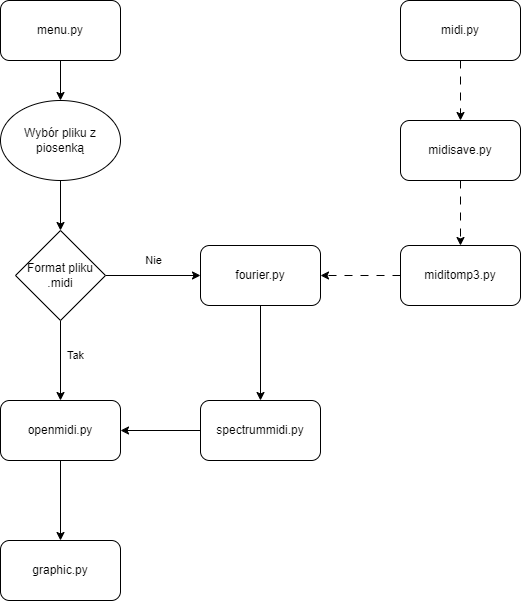
\includegraphics[width=0.69\textwidth]{img/3/diag.png}
  \caption{Diagram przedstawiający architekturę programu}
\end{figure}

\noindent\textbf{Przygotowanie ścieżki dźwiękowej do analizy}

Pierwszym etapem jest odpowiednie przygotowanie ścieżki audio, aby móc przeprowadzić dokładną analizę dźwięku. Najważniejszym elementem przy analizie dźwięku jest widmo ścieżki audio, do którego uzyskania niezbędne jest użycie transformaty Fouriera, a dokładniej STFT. Dzięki czemu można uzyskać macierz amplitud występujących częstotliwości w określonym położeniu w czasie co pozwala na rozpoczęcie analizy ścieżki dźwiękowej.

\begin{figure}[h]
  \centering
  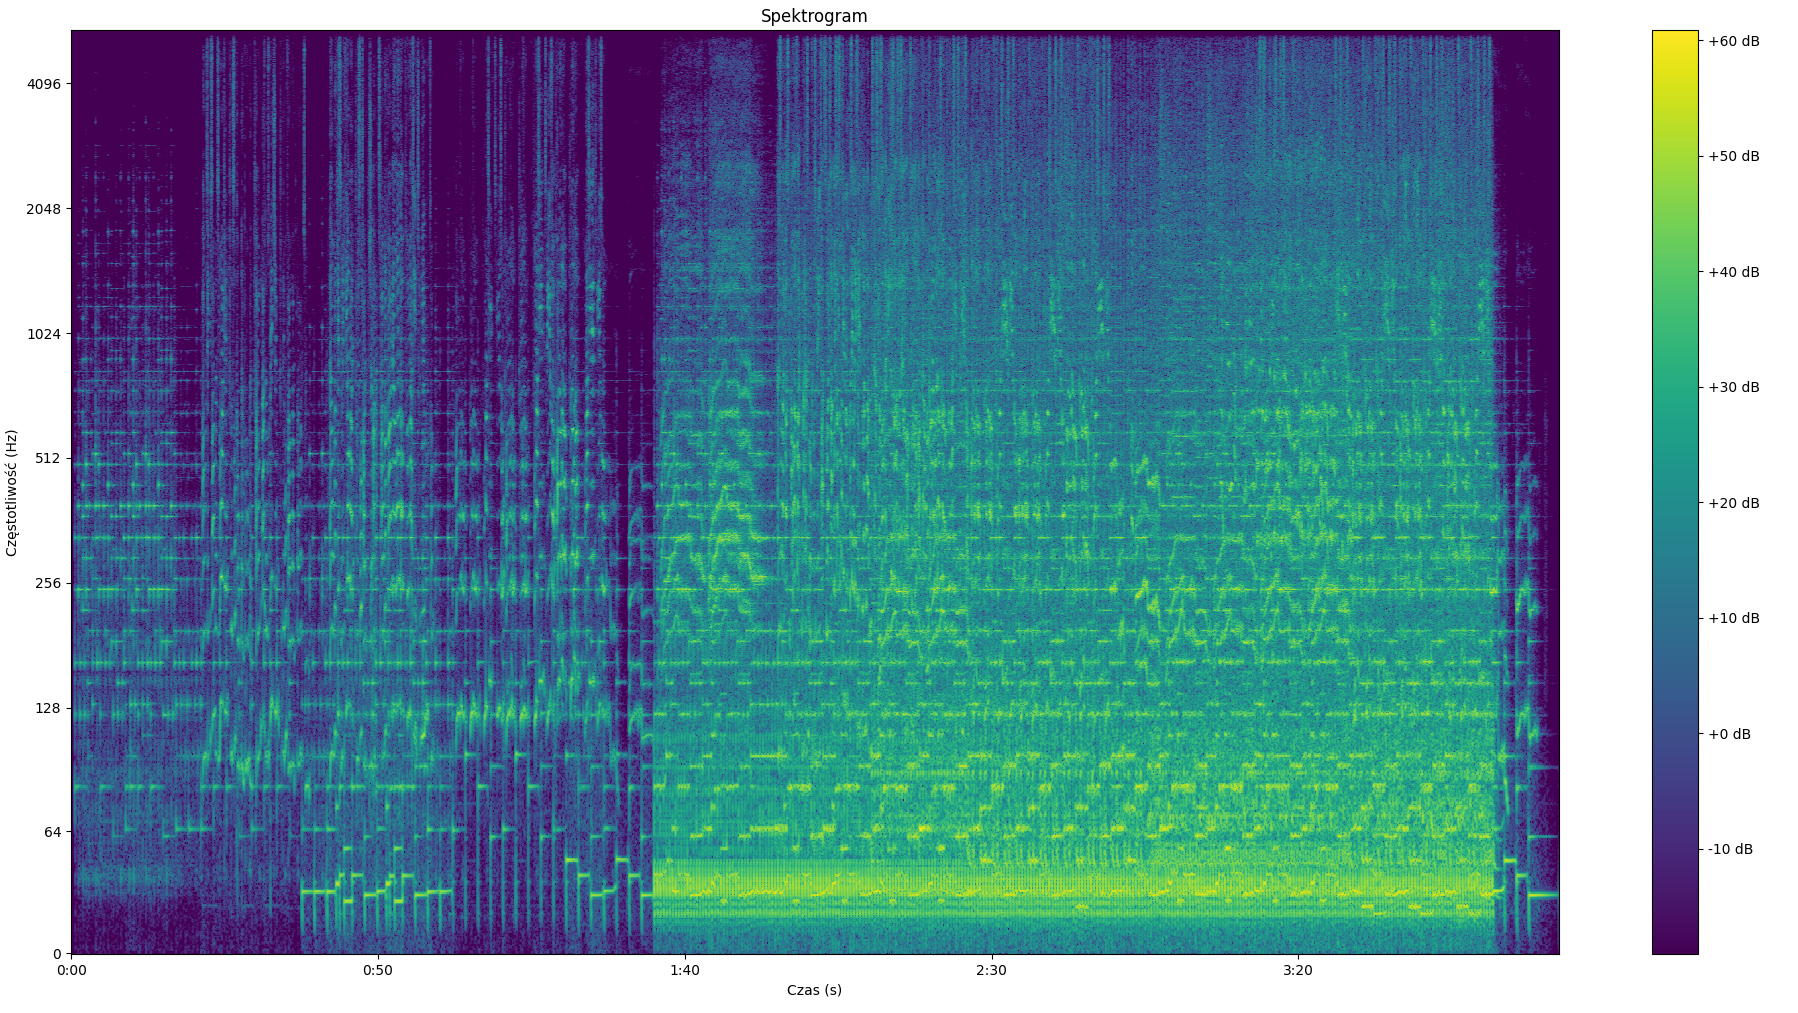
\includegraphics[width=1\textwidth]{img/3/widmo.png}
  \caption{Wykres przedstawiający widmo piosenki Tom Odell - Another Love}
\end{figure}

\noindent\textbf{Synteza dźwięku}

Dźwięk jest tworzony za pomocą syntezy wavetable, ponieważ jest to prosty sposób oraz najbardziej zbliżony do syntezy dźwięku w keyboardzie, gdzie zazwyczaj stosowana jest synteza próbkowa, która odtwarza dźwięki wcześniej nagranych instrumentów. Używając syntezy wavetable, ton zawarty w formacie midi jest podstawiany do gotowych cyfrowych tabel i odpowiednio głośny zależnie od wysokości amplitudy.\\


\noindent\textbf{Interfejs użytkownika}

Użytkownik po uruchomieniu gry ujrzy menu, w którym ma do wyboru rozpoczęcie gry oraz ustawienia. Wciśnięcie przycisku Start powoduje możliwość wyboru pliku audio w formacie mp3/wav, a następnie w tle zostanie przeliczony na plik midi. Zostanie rozpoczęte wyświetlanie grafiki oraz naliczanie punktów na podstawie poprawnego odtwarzania wyświetlanych klawiszy.

\section{Wybór narzędzi i technologii do implementacji}

Za narzędzia posłużył keyboard marki CASIO model CTK-496 \cite{casio_ctk496} oraz interfejs audio MIDI USB marki Roland model UM-ONE MK2 \cite{roland_um_one}, za pomocą których analizowano widmo częstotliwościowe, testowano działanie konwersji na format midi oraz odbieranie sygnału wraz z przeliczaniem punktów uzyskiwanych za poprawne wciskanie klawiszy.

Program został zaprojektowany na system Windows ze względu na jego powszechność wśród użytkowników. Zaimplementowany został w języku Python\cite{python} ze względu na ogrom dostępnych bibliotek oraz ze względu na możliwości w przetwarzaniu dużej ilości danych.

\subsection{Biblioteki Python}

\noindent\textbf{Numpy}\cite{numpy}

To biblioteka do obliczeń numerycznych. Zapewnia efektywne operacje na macierzach, tablicach oraz funkcje matematyczne, umożliwiając pracę z danymi numerycznymi.\\

\noindent\textbf{LibROSA}\cite{librosa}

Jest to biblioteka do analizy sygnałów audio. Umożliwia wczytywanie, przetwarzanie i analizę danych dźwiękowych, oferując narzędzia do ekstrakcji cech dźwiękowych i tworzenia reprezentacji sygnałów. Dostarcza również narzędzia do wizualizacji danych dźwiękowych, umożliwiając wygodne tworzenie wykresów i reprezentacji graficznych sygnałów.\\

\noindent\textbf{Matplotlib}\cite{matplotlib}

Biblioteka służąca do tworzenia wykresów, grafik i wizualizacji danych. Jest często wykorzystywana w analizie danych, naukowych wizualizacjach oraz prezentacji danych ze względu na swoją elastyczność i możliwości dostosowywania wykresów.\\

\noindent\textbf{Pygame}\cite{pygame}

Biblioteka do tworzenia gier i aplikacji multimedialnych. Zawiera moduły do obsługi grafiki, dźwięku, interakcji z użytkownikiem i innych aspektów tworzenia gier.\\

\noindent\textbf{pygame menu}\cite{pygame_menu}

Jest to moduł rozszerzający bibliotekę Pygame, umożliwiający łatwe tworzenie interfejsów użytkownika dla gier i aplikacji napisanych w Pygame.

\newpage
\noindent\textbf{Mido}\cite{mido}

Biblioteka do obsługi danych MIDI. Umożliwia odczyt, zapis, manipulację i tworzenie plików MIDI oraz interakcję z urządzeniami obsługującymi protokół MIDI.\\

\noindent\textbf{midi2audio}\cite{midi2audio}

To narzędzie, które konwertuje pliki MIDI na pliki dźwiękowe (np. WAV, MP3). Używa biblioteki FluidSynth do generowania dźwięku na podstawie plików MIDI.\\

\noindent\textbf{Threading}\cite{threading}

Moduł Pythona umożliwiający tworzenie wielowątkowych aplikacji, gdzie wątki działają równolegle, przydatne do operacji nieblokujących.\\

\noindent\textbf{Tkinter}\cite{tkinter}

Moduł Pythona zawierający standardowy pakiet do tworzenia interfejsów graficznych użytkownika (GUI), oferujący narzędzia do tworzenia okien, przycisków i innych elementów interfejsu.\\

\noindent\textbf{sys}\cite{sys}

Moduł Pythona zapewniający dostęp do niektórych zmiennych i funkcji interakcji ze środowiskiem systemu.\\

\noindent\textbf{os}\cite{os}

Moduł Pythona dostarczający funkcje do interakcji z systemem operacyjnym, takie jak manipulacja plikami, tworzenie katalogów itp.

\subsection{Dodatkowe narzędzia}

\noindent\textbf{FluidSynth }\cite{fluidsynth}

FluidSynth to syntezator dźwięku, który używa plików SoundFont do generowania dźwięku na podstawie plików MIDI. Pliki SoundFont zawierają próbki dźwiękowe różnych instrumentów muzycznych oraz informacje dotyczące sposobu ich odtwarzania. FluidSynth jest narzędziem open-source, które umożliwia odczyt plików MIDI i syntezę dźwięku na ich podstawie. Dzięki temu użytkownik może generować dźwięki różnych instrumentów muzycznych, manipulować parametrami dźwięku, takimi jak wibrato, głośność czy barwa, co jest przydatne w procesie komponowania, edycji dźwięku czy też w aplikacjach muzycznych.

\newpage

\noindent\textbf{FFmpeg} \cite{ffmpeg}

FFmpeg to zestaw narzędzi do nagrywania, konwersji i strumieniowania plików audio oraz wideo. Jest to oprogramowanie open-source, które działa na wielu platformach, umożliwiając manipulację multimediów. Za jego pomocą można wykonywać różne operacje, takie jak konwersja formatów plików, kompresja, ekstrakcja strumieni wideo i audio, łączenie plików, nagrywanie strumieni czy też aplikowanie efektów. FFmpeg obsługuje dużą liczbę formatów plików multimedialnych i oferuje szeroki zakres opcji konfiguracyjnych, co sprawia, że jest powszechnie używany w edycji wideo i audio, transmisji strumieniowej, produkcji multimediów oraz jako silnik w wielu aplikacjach multimedialnych.

\section{Algorytm}

\subsection{Analiza ścieżki dźwiękowej}

Wykres spektrogramu ukazuje dominujące częstotliwości oraz ich położenie, natomiast oprócz samych głównych dźwięków widoczna jest ich powtarzalność z oktawy na oktawę wraz ze wzrostem częstotliwości. Są to składowe harmoniczne, które nadają dźwięku charakterystyczną barwę oraz głębię. Dzięki nim piosenka staje się bogatsza oraz sprawiają, że analiza dźwięku jest znacznie cięższa. Powodem tego jest ich zróżnicowanie, co uniemożliwia ich jednoznaczną identyfikację. Możliwe jest również powielenie się składowych harmonicznych z głównym dźwiękiem, co powoduje że główny dźwięk może zostać uznany jako składowa harmoniczna i nie zostać wykryty.
\subsection{Detekcja tonów}

\noindent\textbf{Główne założenia detekcji}

Ton może zostać wykryty za pomocą tylko jednej zmiennej, mianowicie amplitudy, a każdemu z nich odpowiada konkretna częstotliwość (Tab. 2.1). Rozpoznawanie dźwięków rozpocznie się od przechodzenia po kolei każdej zdefiniowanej w tabeli częstotliwości po czasie. Miejsca, w których amplituda jest odpowiednio wysoka oznacza znalezienie poszukiwanego tonu. Algorytm początkowo poszukuje komórki, gdzie amplituda osiągnie maksimum lokalne, którego wartość jest większa od ustalonego progu detekcji. Następnie cofa się w czasie, aż do znalezienia minimum lokalnego, co oznacza wykrycie rozpoczęcia się danego dźwięku. Po tym algorytm idzie dalej od maksimum lokalnego szukając minimum lokalnego. Jeśli zostanie znalezione, a amplituda nadal będzie wyższa niż ustalony próg, to oznacza znalezienie miejsca, w którym ten sam klawisz został ponownie naciśnięty i rozpoczął się ponowny wzrost amplitudy w czasie. Natomiast jeśli minimum nie zostało znalezione, zanim amplituda przekroczyła granicę podtrzymania tonu, zostaje zapisana informacja o zakończeniu wciśnięcia danego dźwięku.\\




\noindent\textbf{Próg graniczny detekcji}

Wnioskując z uprzednich założeń, wykrywanie tonów zależy głównie od ustalonej wartości progu detekcji. Do jego ustalenia potrzebny jest zakres amplitud, jaki występuje w danej ścieżce muzycznej. Próg należało dobrać tak, aby zostały wykryte tony występujące w danym utworze, a nie zostały wykryte żadne, które w nim nie występują. 

Pierwsza metoda wyznaczania progu wykonuje to z użyciem wartości maksymalnej amplitudy pomnożonej przez współczynnik ustalony w zależności od charakterystyki utworu. 
Jednakże piosenki nie są jednostajne, składają się z fragmentów, gdzie wahania amplitudy dźwięków są względnie stałe, jak i również z fragmentów wyciszenia oraz nasilenia. 

Uwzględniając to powstała druga metoda wyznaczając próg detekcji używając maksymalnej amplitudy oraz średniej, które zostały zsumowane i wymnożone przez współczynniki.

Niemniej jednak w zależności od barwy oraz charakterystyki utworu dźwięki różnią się amplitudą nie tylko na przestrzeni czasu, ale również częstotliwości. Metoda trzecia zatem odzwierciedla szukanie tonów przez człowieka na wykresie widma, czyli doszukiwanie się poziomych linii o wyższej amplitudzie niż najbliższe otoczenie. Otoczenie w zakresie częstotliwości, będzie obejmowało zauważalne zwiększenie amplitudy przez dany ton, a w zakresie czasu kilkaset milisekund.\\

\noindent\textbf{Składowe harmoniczne}

Główną przeszkodą w poprawnym rozpoznawaniu tonów są składowe harmoniczne. Jak zostało wcześniej wspomniane mogą przykryć główny dźwięk, bądź go imitować. 

Składowe harmoniczne występują na częstotliwościach, które są wielokrotnościami częstotliwości, od której pochodzą i są znacząco widoczne na dwukrotności, trzykrotności oraz czterokrotności tejże częstotliwości. Dwukrotność oraz czterokrotność nie zmienia drastycznie wybrzmienia, ponieważ to jest ten sam ton tylko oktawę i dwie oktawy wyżej, czyli dwanaście i dwadzieścia cztery półtony. Natomiast trzykrotność częstotliwości znacząco może zmienić brzmienie, ponieważ przykładowo dźwięk A na drugiej oktawie ma częstotliwość 110Hz. Trzykrotność tej częstotliwości to 330Hz, która jest na tyle blisko dźwięku E na czwartej oktawie (którego częstotliwość wynosi 329.63Hz), że znacząco wpływa na podwyższenie amplitudy i może powodować że dźwięk może zostać błędnie zidentyfikowany. Błąd między harmoniczną trzykrotną, a najbliższym tonem to zaledwie około jeden procent błędu względem kolejnego tonu. 

Niestety wiele utworów muzycznych składa się z sekwencji, gdzie grany ton jest grany również o dwanaście, dziewiętnaście i dwadzieścia cztery półtony. Dźwięki harmoniczne również nie mają zależności w postaci amplitudy, czasem potrafią mieć większy poziom decybeli, niż dźwięk z którego pochodzą, a więc nie ma żadnej zasady, którą byłaby możliwość kierowania się, a co za tym idzie próbując usunąć składowe harmoniczne, najprawdopodobniej zostaną usunięte główne dźwięki.

Próba usunięcia dźwięków harmonicznych polega na sprawdzaniu przy każdym znalezionym dźwięku, czy w bardzo małym zakresie przed jego rozpoczęciem, nie rozpoczął się dźwięk niższy o dwanaście, dziewiętnaście i dwadzieścia cztery półtony.

        \chapter{Implementacja}
\vspace{-20pt}

Rozdział ten opisuje w jaki sposób zostały zrealizowane założenia projektu z podziałem na poszczególne pliki. Przedstawia również dokładnie i szczegółowo opisane rozwiązania implementacyjne zadań, na które projekt został podzielony.

\section{Odebranie sygnału wyjściowego z keyboardu i zapis}

\noindent\textbf{midi.py}

Odpowiada za znalezienie odpowiedniego urządzenia spośród wejściowych portów, odbieranie sygnału muzycznego oraz za zapis do zmiennej odbieranego sygnału przez ustalony czas.

Z użyciem biblioteki Pygame \cite{pygame} zostaje znaleziona ilość portów i sprawdza podłączone do nich urządzenia. Wybiera właściwe oraz wybiera sygnał wyjściowy urządzenia. Gdy takowe nie zostanie znalezione, zwraca komunikat o nieznalezieniu żadnego wejścia midi. Natomiast jeśli zostanie znalezione, tworzy macierz za pomocą biblioteki NumPy \cite{numpy} o rozmiarze skali dwunastotonowej na 10, czyli ilość oktaw obejmującą zakres częstotliwości zawierający częstotliwości praktycznie wszystkich instrumentów muzycznych. Macierz ta służy do zapisu czasu wciśnięcia konkretnego klawisza, ze względu na charakterystykę przychodzenia sygnału z keyboardu, a mianowicie dostarczaniu sygnału po wciśnięciu klawisza oraz po jego odpuszczeniu, natomiast czas jest naliczany za pomocą Pygame \cite{pygame}. Sygnał był odbierany przez czas, określony w zależności od potrzeb. Zawiera informacje dotyczące kanału, z którego pochodzi dźwięk, nutę, amplitudę, czas oraz interakcje z klawiszem. Następnie tak jak w formacie midi zapisywana jest akcja o wciśnięciu konkretnych klawiszy i czas oraz potem o ich odpuszczeniu.\\

\noindent\textbf{midisave.py}

Służy do zapisu uprzednio zebranego sygnału do pliku w formacie midi.
Uruchamia plik midi.py, z którego odebranej sekwencji czas jest przeliczany z bezwzględnego na względny względem siebie, tak jak odczytuje to format midi. Za pomocą biblioteki Mido \cite{mido} ta kombinacja jest konwertowana i zapisywana jako plik w formacie midi.\\

\newpage
\noindent\textbf{miditomp3.py}

Użycie FluidSynth \cite{fluidsynth} i biblioteki midi2audio \cite{midi2audio} pozwoliło zmienić uzyskany wcześniej plik midi na plik w formacie mp3 z użyciem dowolnie wybranego soundfontu, a zatem metody syntezy wavetable.\\

Użycie powyższych skryptów umożliwiło pozyskanie pliku z własnej gry, a co za tym idzie testowanie własnoręcznie zagranych sekwencji, a zarazem dokładniejsze zrozumienie cech dźwięku i sprawdzenie działania reszty programu.

\section{Uzyskanie spektrogramu przy użyciu transformaty Fouriera}

\noindent\textbf{fourier.py}

Ten element odpowiada za utworzenie widma wybranego pliku audio. Z użyciem biblioteki os odczytywana jest ścieżka do wybranego pliku, a następnie za pomocą biblioteki LibROSA \cite{librosa} ze wskazanego pliku odczytywana jest częstotliwość próbkowania oraz wektor reprezentujący amplitudę całego sygnału audio. Następnie określona wartość  $n\_fft$ wynoszące $2^{14}$ i $hop\_length$ wynoszące $2^8$. Wartości te oznaczają odpowiednio liczbę punktów próbkowania użytych do każdej ramki oraz ilość próbek między kolejnymi ramkami.

W dalszym kroku za pomocą funkcji librosa.stft obliczana jest transformata Fouriera z wczytanego uprzednio sygnału audio i ustalonych wartości, czego efektem końcowym jest uzyskanie macierzy amplitud. Następuje konwersja na decybele i zostaje wyświetlony oraz zapisany za pomocą biblioteki Matplotlib \cite{matplotlib} wykres powstałego widma, gdzie oś x reprezentuje czas, oś y częstotliwości, a natężenie koloru odpowiada za głośność.

\section{ Analiza uzyskanego widma i konwersja na plik w formacie midi}

\noindent\textbf{spektrummidi.py}

Użycie pliku fourier.py pozwala na przekształcenie widma ścieżki dźwiękowej za pomocą algorytmu na format muzyczny midi. 
Algorytm ten na początek otrzymuje widmo pliku audio w postaci macierzy amplitud oraz wektor częstotliwości i wektor czasu. Zawarta lista z częstotliwościami odpowiadającymi danym tonom (Tab. 2.1) jest porównywana do częstotliwości otrzymanych ze skryptu fourier.py i zostają zapisane indeksy częstotliwości, które są najbliżej częstotliwości szukanych. Lista ta została zmodyfikowana, użyte zostały częstotliwości z najwyższej oktawy, a następnie kolejno dzielone przez 2, aby uzyskać dokładniejsze niższe częstotliwości. Porównywanie polega na przechodzeniu po wszystkich częstotliwościach z tabeli, których jest 12 dźwięków przez 9 oktaw, czyli 108, a następnie po wszystkich częstotliwościach z użycia transformaty Fouriera sprawdzając po kolei, dla której wartości bezwzględna różnica będzie najmniejsza. 	
Po uzyskaniu indeksów pożądanych częstotliwości z widma może się odbyć przeszukiwanie macierzy amplitud po tych częstotliwościach. Nim ten proces się rozpocznie, zostaje znaleziona wartość maksymalna występującej amplitudy, a następnie z użyciem biblioteki NumPy \cite{numpy} tworzona jest lista list, do której zapisywane będą znalezione przez algorytm dominujące dźwięki. Sam algorytm zaś przeszukuje każdy ton po czasie tak jak to zostało opisane w podrozdziale 3.3. Algorytm.
Po przeszukaniu całego sygnału, uzyskane wartości zostają zapisane za pomocą skryptu midisave.py, co pozwala na odtworzenie wyniku końcowego.

\section{Powstawanie synthesii ze ścieżki audio w formacie midi}

\noindent\textbf{openmidi.py}

Po wskazaniu ścieżki audio następuje przekształcenie wybranej piosenki z formatu midi za pomocą biblioteki mido \cite{mido} na listę słowników.\\

\noindent\textbf{graphic.py}

Główny skrypt odpowiadający za wyświetlanie synthesii rozpoczyna działanie od zdefiniowania funkcji. 

Funkcja \_\_init\_\_() rozpoczyna się inicjalizacją wszystkich modułów dostarczanych przez bibliotekę Pygame \cite{pygame}. Następnie zostają zebrane i ustawione dane o rozdzielczości monitora, dodane flagi ustawiające pełny ekran i podwójne buforowanie, co wspomaga optymalizację. Natomiast druga funkcja run() zawiera w sobie główną pętlę, która odpowiada za obliczanie i wyświetlanie oraz zawiera w sobie dwie funkcje zagnieżdżone.

Funkcja convert\_song() odpowiada za przekonwertowanie listy zawierającej akcje dotyczące każdego pojedynczego tonu. Konwersja polega na połączeniu akcji rozpoczęcia trwania tonu i akcji jego zakończenia na ton, który zawiera czas trwania. Konwersja powoduje również zmianę z czasu względnego, jaki występuje w formacie midi, na czas bezwzględny. Po tym następuje sortowanie tonów względem czasu i zwrócone w postaci listy do wyświetlenia. Natomiast zadaniem drugiej funkcji key\_parametres() jest przekształcenie tonu na klawisz, zwracając jego miejsce położenia, szerokość oraz kolor, dla półtonów czarny i dla pełnych tonów biały.

Funkcja player\_info sprawdza, czy istnieje plik tekstowy z danymi gracza. Jeśli tak to sprawdza, czy zawiera informacje o ilości punktów uprzednio zgromadzonych przez gracza. Jeśli nie to tworzy plik tekstowy o nazwie uprzednio podanej przez gracza.

\newpage
Kolejnym krokiem jest przygotowanie zmiennych używanych w głównej pętli. Zależnie od ilości oktaw i szerokości ekranu odpowiednio wyliczana jest szerokość białych klawiszy.

\begin{equation}
\[
w = \frac{s}{7 \cdot o}
\]
\end{equation}

gdzie:
\begin{itemize}
    \item \(w\) jest szerokością białego klawisza,
    \item \(s\) jest szerokością ekranu,
    \item \(o\) jest liczbą oktaw.
\end{itemize}

Następnie na podstawie pliku midi.py zostaje przechwycony sygnał z keyboardu, co pozwala na porównywanie gry użytkownika względem włączonej piosenki. Najważniejszą częścią jest główna pętla, która rozpoczyna się od jednorazowego utworzenia całej klawiatury. Najpierw są tworzone białe klawisze, następnie czarne po wszystkich oktawach. 

\begin{figure}[h]
  \centering
  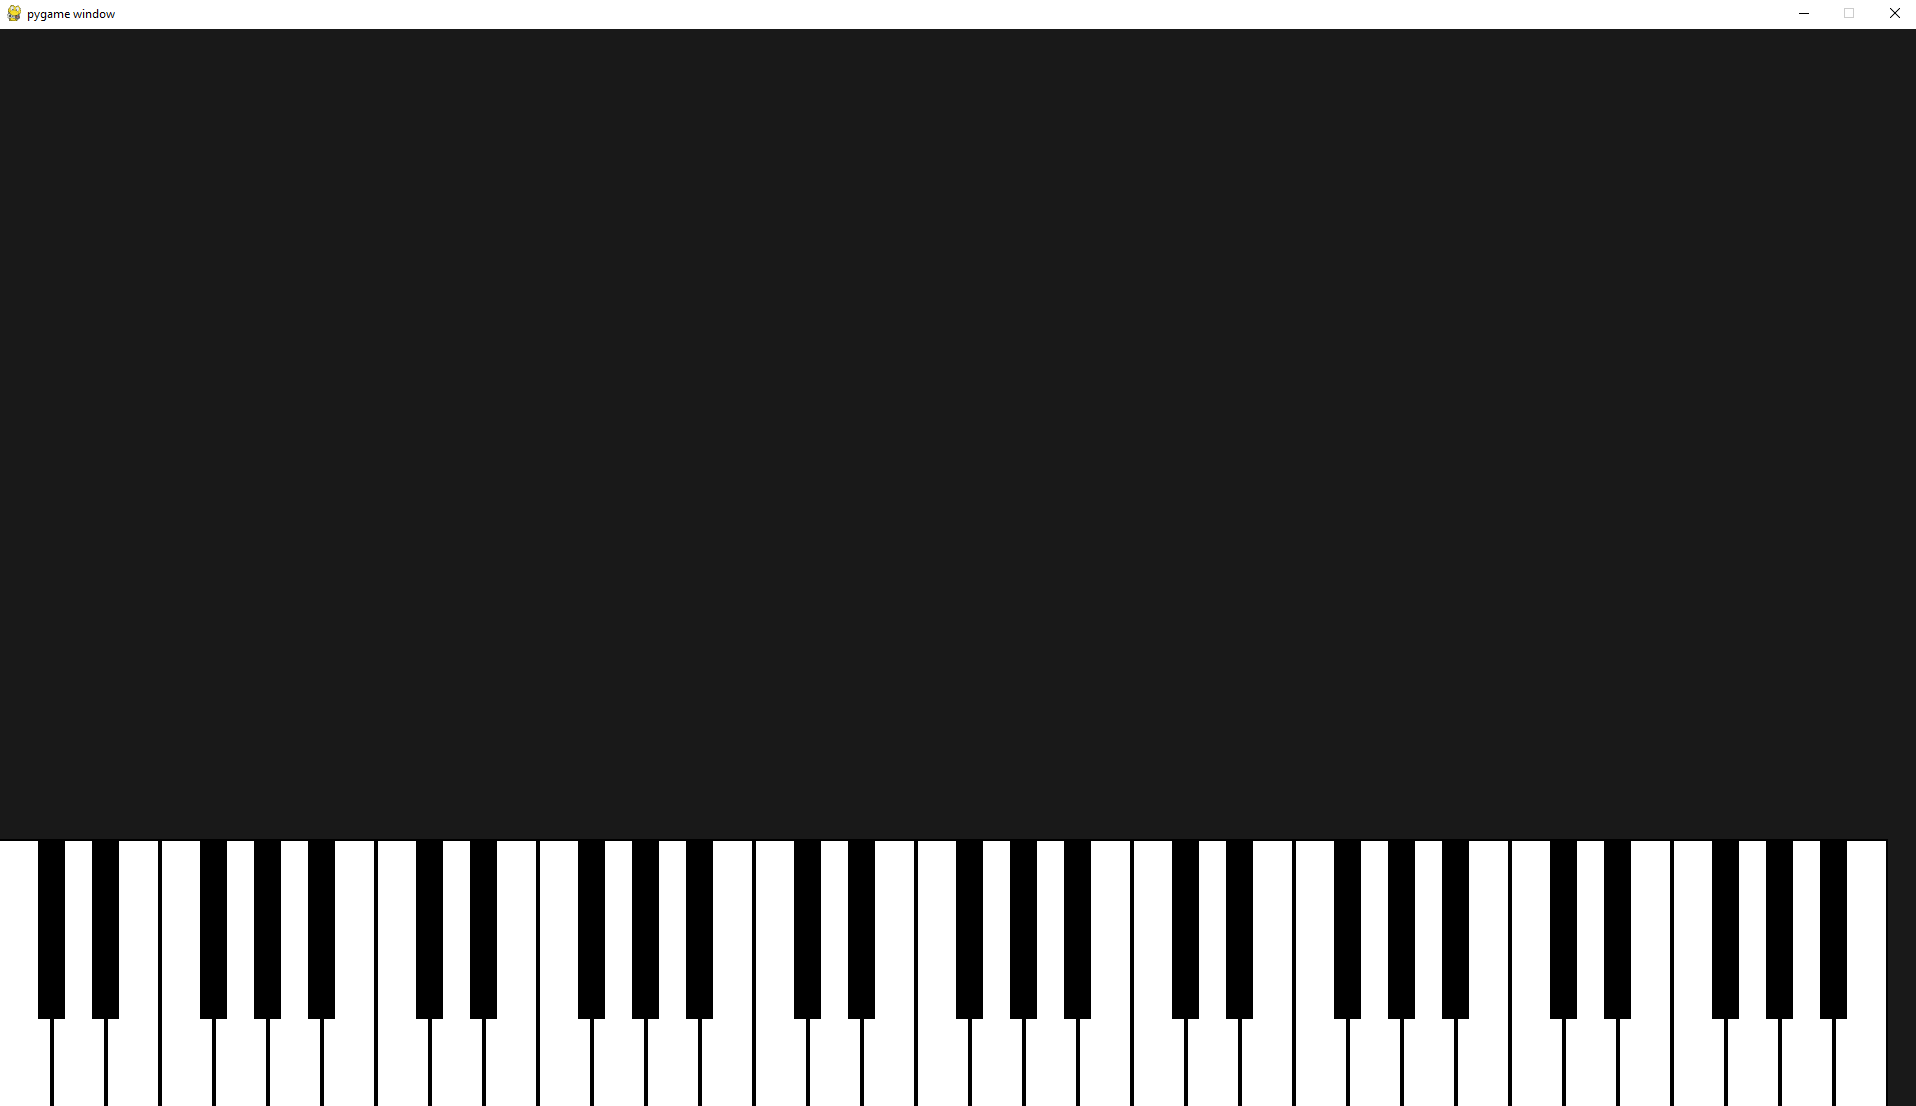
\includegraphics[width=1\textwidth]{img/4/klawiatura.png}
  \caption{Wygląd rozpoczętej gry}
\end{figure}

W kolejnym kroku program sprawdza, czy przyszedł sygnał pochodzący z interakcji użytkownika z keyboardem. Potem następuje część odpowiedzialna za wyświetlanie całego utworu muzycznego. Porównując czas pierwszego tonu w liście z aktualnym, jest on usuwany z aktualnej i przenoszony do listy wyświetlanych tonów.

Następnie pętla przechodząca po tejże liście oblicza wysokość na ekranie każdego tonu ograniczając go, aby na początku nie był widoczny na ekranie, a na wysokości rozpoczynania się klawiatury został usunięty z listy wyświetlanych tonów. Długość natomiast początkowo jest proporcjonalna do czasu trwania tonu, a gdy ma zacząć zakrywać klawiaturę, jest adekwatnie zmniejszana. W tym samym momencie zaczyna się podświetlać klawisz, który użytkownik powinien nacisnąć, a gdy wygasa, część klawiatury podświetlanego klawisza zostaje nadbudowana. Kolejna część jest odpowiedzialna za wyświetlanie synthesii z użyciem pygame.draw.rect, co pozwala na wyświetlenie prostokątnego kształtu z zadanym wcześniej kolorem, szerokością, długością oraz położeniem. Szerokość wyświetlanego kształtu jest zależna od tego, czy to półton czy cały ton oraz szerokość położenia na ekranie zależna od wysokości tonu. Końcówka wyświetlanego tonu zostaje nadbudowywana kolorem tła, aby po jego zakończeniu nie został po nim widoczny ślad, który przeszkadzałby w rozczytywaniu kolejnych tonów.

\begin{figure}[h]
  \centering
  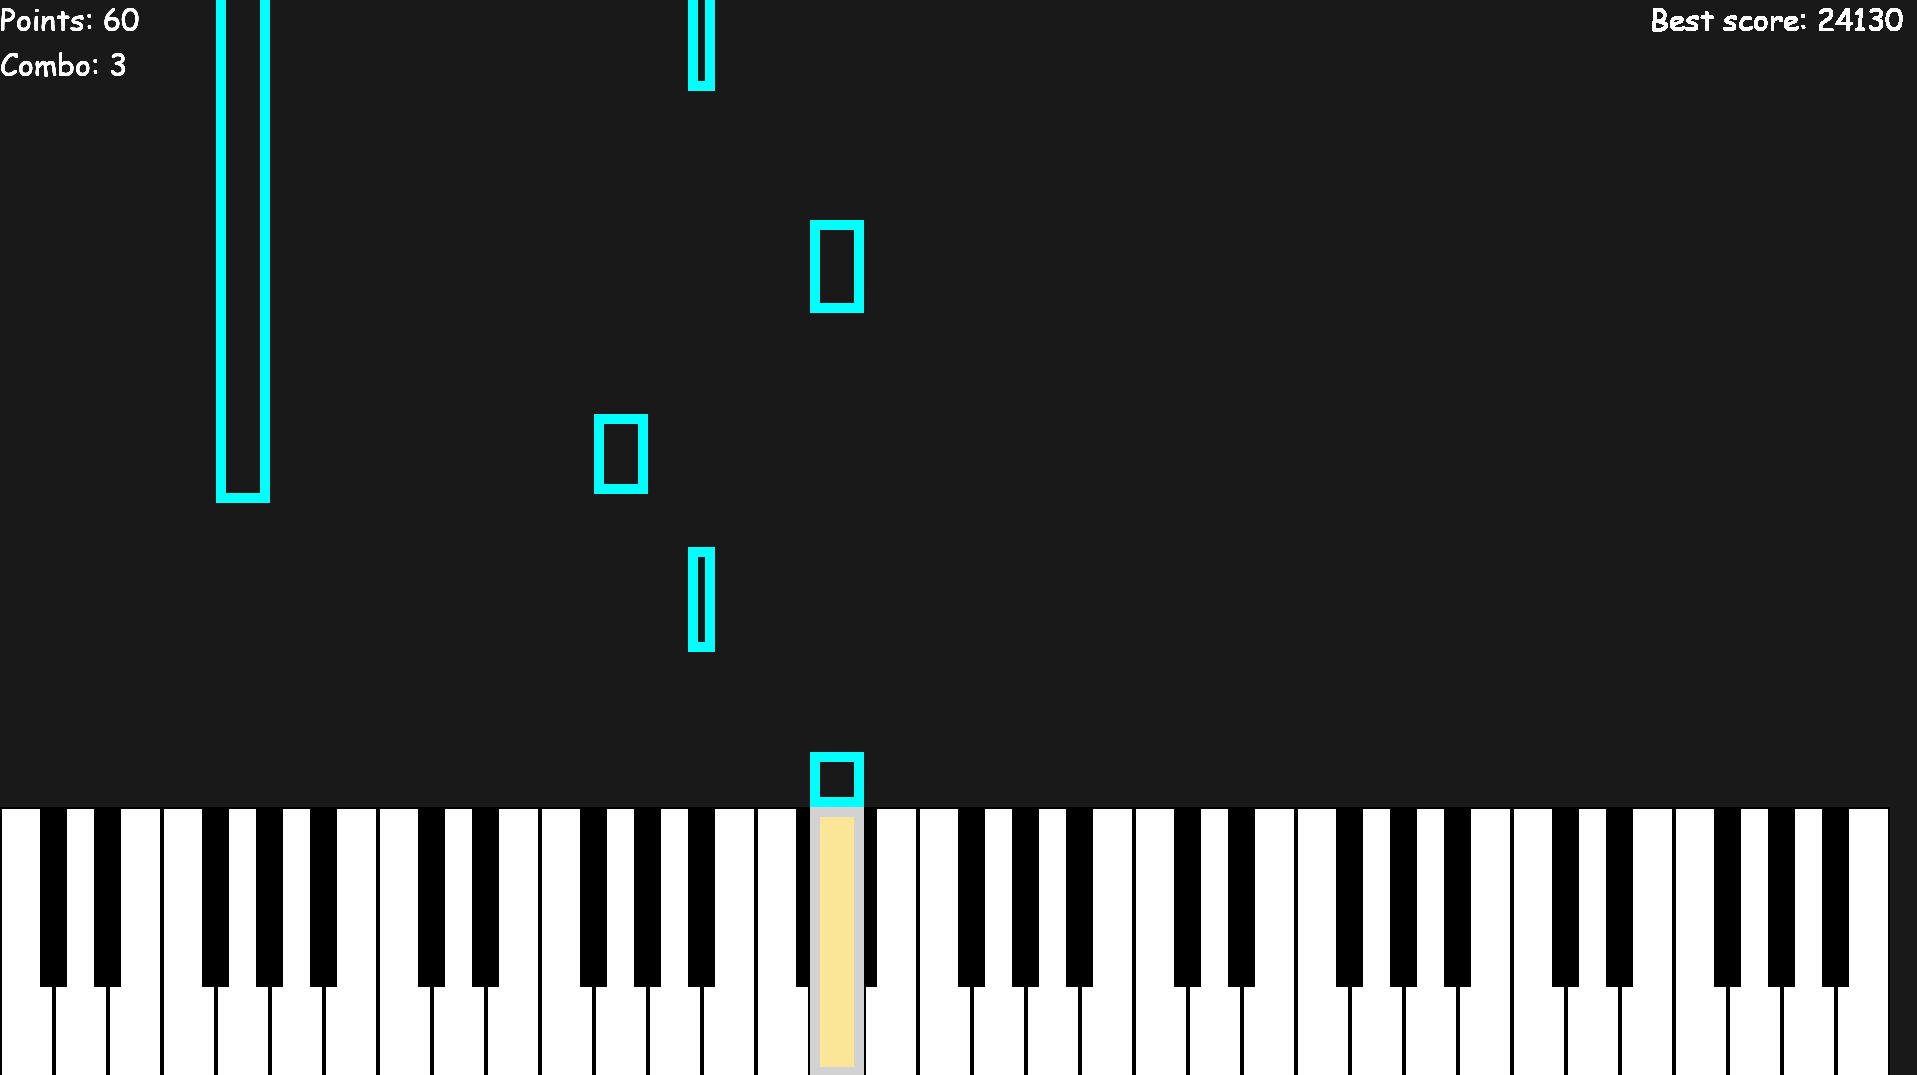
\includegraphics[width=1\textwidth]{img/4/synthesia.png}
  \caption{Wyświetlająca się synthesia}
\end{figure}

Ostatnią częścią dotyczącą synthesii jest zliczanie punktów za poprawne powtarzanie sekwencji na instrumencie. Gdy dany klawisz się podświetla i użytkownik naciśnie go w odpowiednim czasie, zostaną dodane punkty przemnożone przez mnożnik zwiększający się o 1 za każdym poprawnym naciśnięciem oraz zerujący się, gdy któryś klawisz nie zostanie wciśnięty, bądź zostanie naciśnięty nieprawidłowy klawisz. Naliczane punkty są na bieżąco wyświetlane w lewym górnym rogu ekranu gry  (por. Rys. 4.2), a w prawym górnym rogu widnieje najlepszy wynik uzyskany uprzednio przez gracza.

Główna pętla kończy się dodaną funkcjonalnością klawiszy, które pozwalają na rozpoczęcie wyświetlania synthesii oraz na wyjście z niej. Przy opuszczeniu programu, jeśli gracz uzyskał więcej punktów niż swój rekord, bądź nie posiadał jeszcze wyniku dla danej piosenki, ilość zebranych punktów zostaje zapisana do pliku profilu gracza.

\begin{figure}[h]
  \centering
  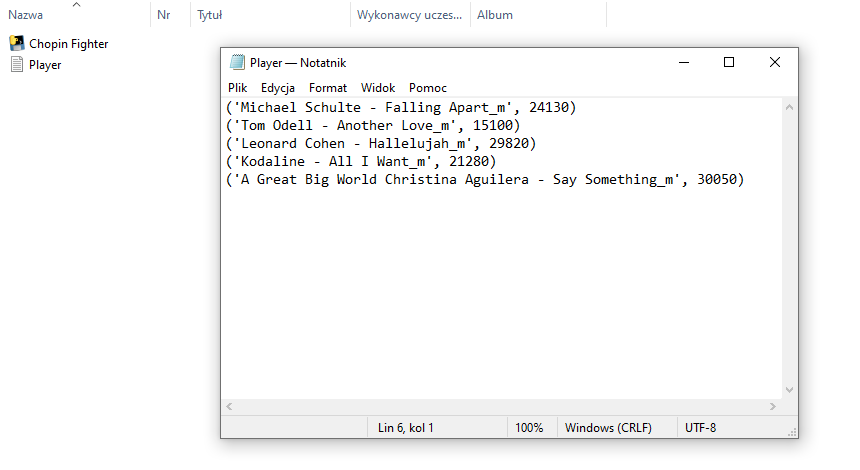
\includegraphics[width=1\textwidth]{img/4/wyniki.png}
  \caption{Stworzony plik z profilem gracza zawierający informacje o najlepszych wynikach}
\end{figure}

\section{Scalenie projektu}

\noindent\textbf{menu.py}

Do scalenia wszystkich plików ważnym elementem było stworzenie funkcjonalnego menu, które będzie zarazem estetyczne i przyjemne dla oka.
Niezbędne okazały się biblioteki Pygame \cite{pygame} oraz pygame-menu \cite{pygame_menu}. Program zawiera w sobie kilka funkcji, które poprzedza zainicjowanie użycia wcześniej wymienionych bibliotek. Na sam początek zostaje zebrana informacja o rozdzielczości ekranu, a następnie utworzone całe menu.

\begin{figure}[h]
  \centering
  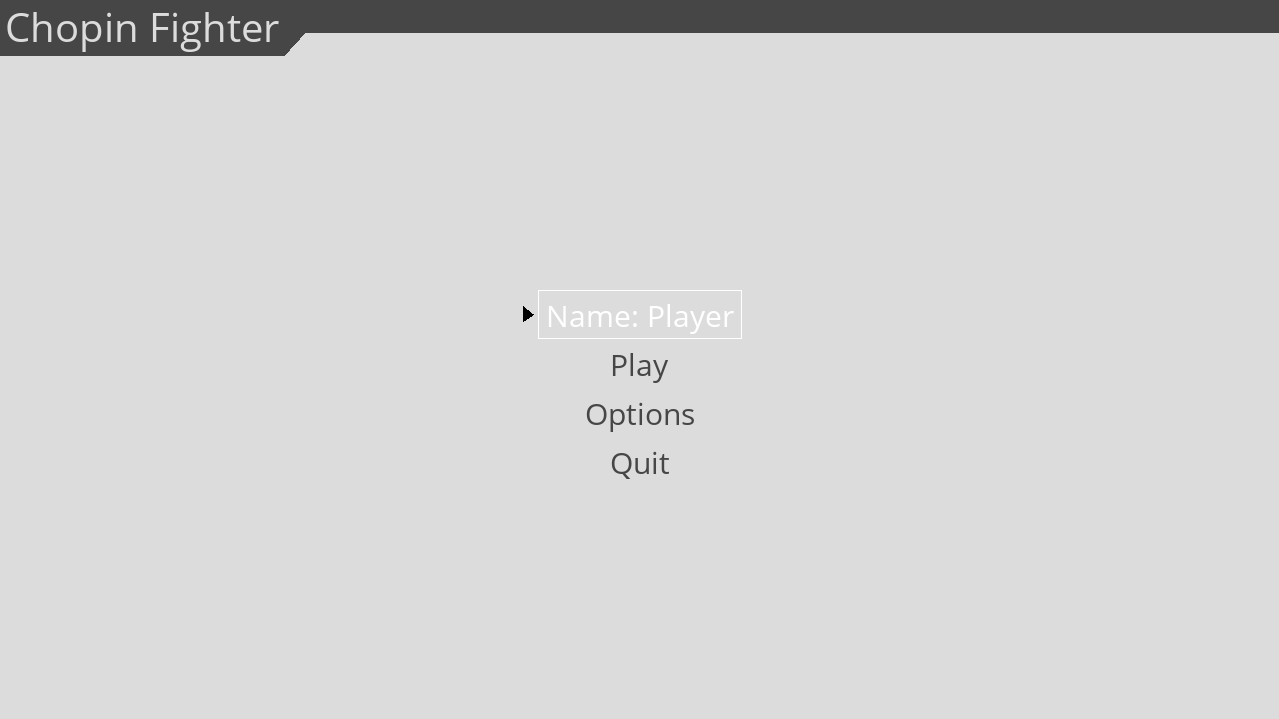
\includegraphics[width=0.88\textwidth]{img/4/menu.png}
  \caption{Menu gotowego programu}
\end{figure}

W głównej pętli menu zbierane są informacje o akcji użytkownika oraz odświeżanie grafiki, przez co menu staje się funkcjonalne. Na początkowym ekranie (por. Rys. 4.4.) widnieją trzy przyciski. Przycisk Quit uruchamia funkcję zatrzymującą główną pętlę oraz kończącą proces biblioteki Pygame \cite{pygame}. Przycisk Options otwiera menu opcji, w którym jest do wyboru rozdzielczość, w jakiej program ma działać. Wybór jest możliwy spośród najczęściej występujących rozdzielczości oraz nominalnej wykrytej na początku. Menu opcji daje możliwość wyboru trudności granego utworu, lecz jest to funkcja koncepcyjna. Wyjść bez zmiany ustawień można przyciskiem w prawym górnym rogu.

\begin{figure}[h]
  \centering
  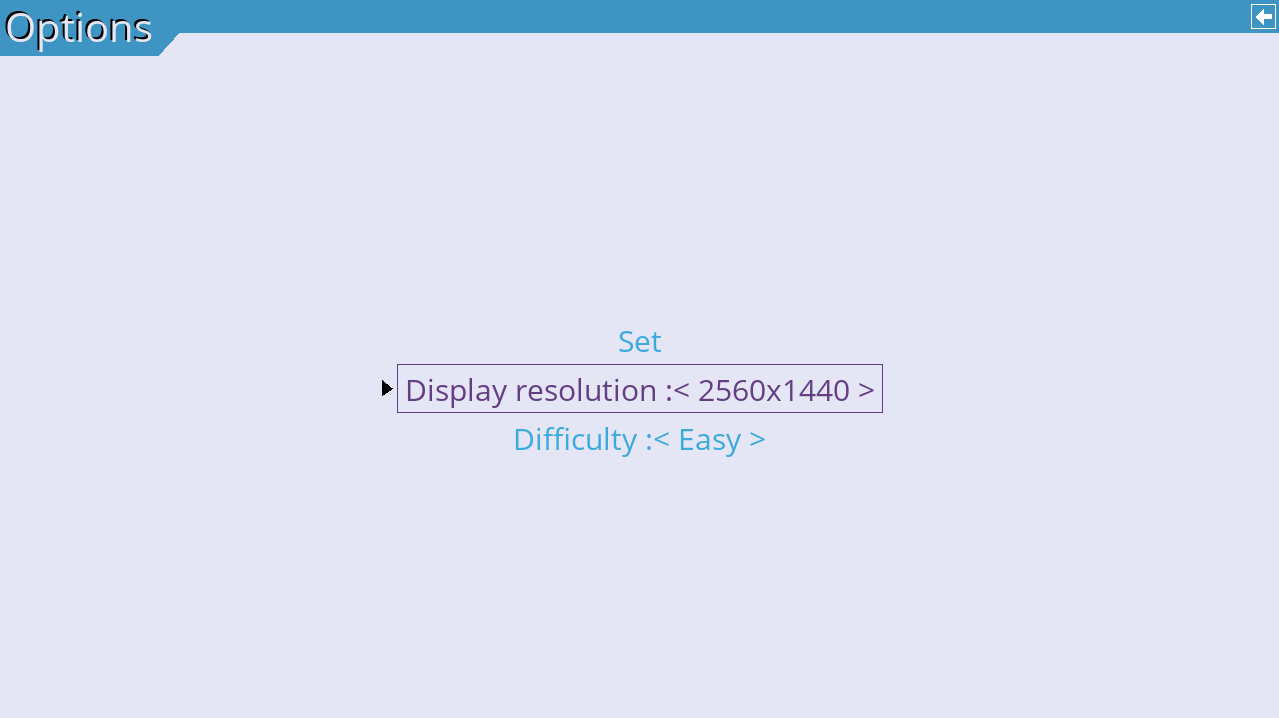
\includegraphics[width=0.88\textwidth]{img/4/opcje.png}
  \caption{Menu opcji}
\end{figure}

\newpage
Przycisk Play powoduje otwarcie się okna do wyboru pliku muzycznego, który w zależności od rozszerzenia pliku uruchomi wyświetlanie synthesii albo analizę pliku muzycznego, a następnie konwersję na format midi, po której dopiero nastąpi wyświetlenie synthesii.

\begin{figure}[h]
  \centering
  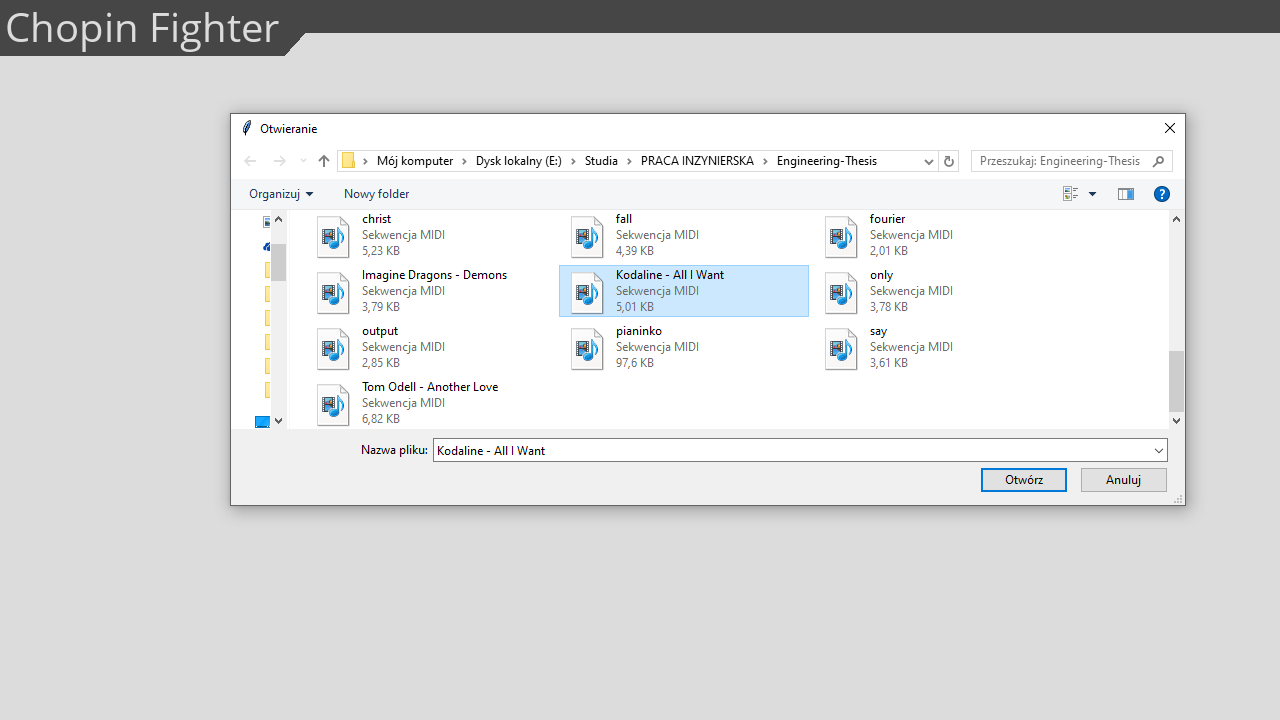
\includegraphics[width=1\textwidth]{img/4/wybor.png}
  \caption{Wybór pliku audio}
\end{figure}
        \chapter{Testy i analiza wyników}
\vspace{-25pt}
\section{ Opis przeprowadzonych testów funkcjonalnych systemu}
Testom podlegać będzie wyjściowa ścieżka audio powstająca w wyniku działania algorytmu analizującego widmo piosenki wejściowej. Wyjściowa ścieżka audio będzie porównywana z wejściową piosenką według wybranych kryteriów sprawdzających jakość uzyskanej piosenki:\\
• poprawność rozpoznanych tonów,\\
• czas rozpoczęcia i zakończenia znajdowanych tonów,\\
• czy wszystkie wyszukane tony występują w wejściowym utworze.

Algorytmy analizy dźwięku zostały sprawdzone na trzech przykładowych piosenkach, które w oryginale głównie składają się z gry na instrumencie klawiszowym oraz wokalu:\\
• A Great Big World - Say Something \cite{say_something},\\
• Leonard Cohen - Hallelujah \cite{hallelujah},\\
• Michael Schulte - Falling Apart \cite{falling_apart}.

Następnie każda z nich została poddana testom w trzech różnych wersjach:\\
• piosenki powstałej z syntezy pliku z formatu midi na format wav,\\
• piosenki zagranej na instrumencie klawiszowym typu pianino, bądź fortepian \cite{say_something_piano_cover}\cite{hallelujah_piano_cover}\cite{falling_apart_piano_cover},\\
• oryginalnej piosenki wraz z wokalem.

Każda z powyższych wersji została sprawdzona przez trzy metody wyliczania progu detekcji. Poza algorytmem detekcji dźwięku testom podlega również wyświetlanie synthesii.

\newpage
\section{Testy}

\subsection{Pierwsza metoda detekcji głównych składowych utworu}

Metoda polegająca na wyznaczeniu progu granicznego z użyciem maksymalnej wartości amplitudy pomnożonej przez współczynnik m wyznaczony na podstawie wykresu. Dobierając odpowiednie wartości parametrów do wyznaczania wartości granicznej amplitudy najlepsze efekty dawała metoda łokciowa, która polegała na znalezieniu zgięcia odpowiadającemu nagłemu braku spadku ilości znajdowanych przez algorytm tonów. Dobrze jest to widoczne na syntetycznie stworzonej ścieżce dźwiękowej widocznej w środkowej kolumnie wykresu, gdzie każdy główny dźwięk ma małe oscylacje amplitudy.

\begin{figure}[h]
  \centering
  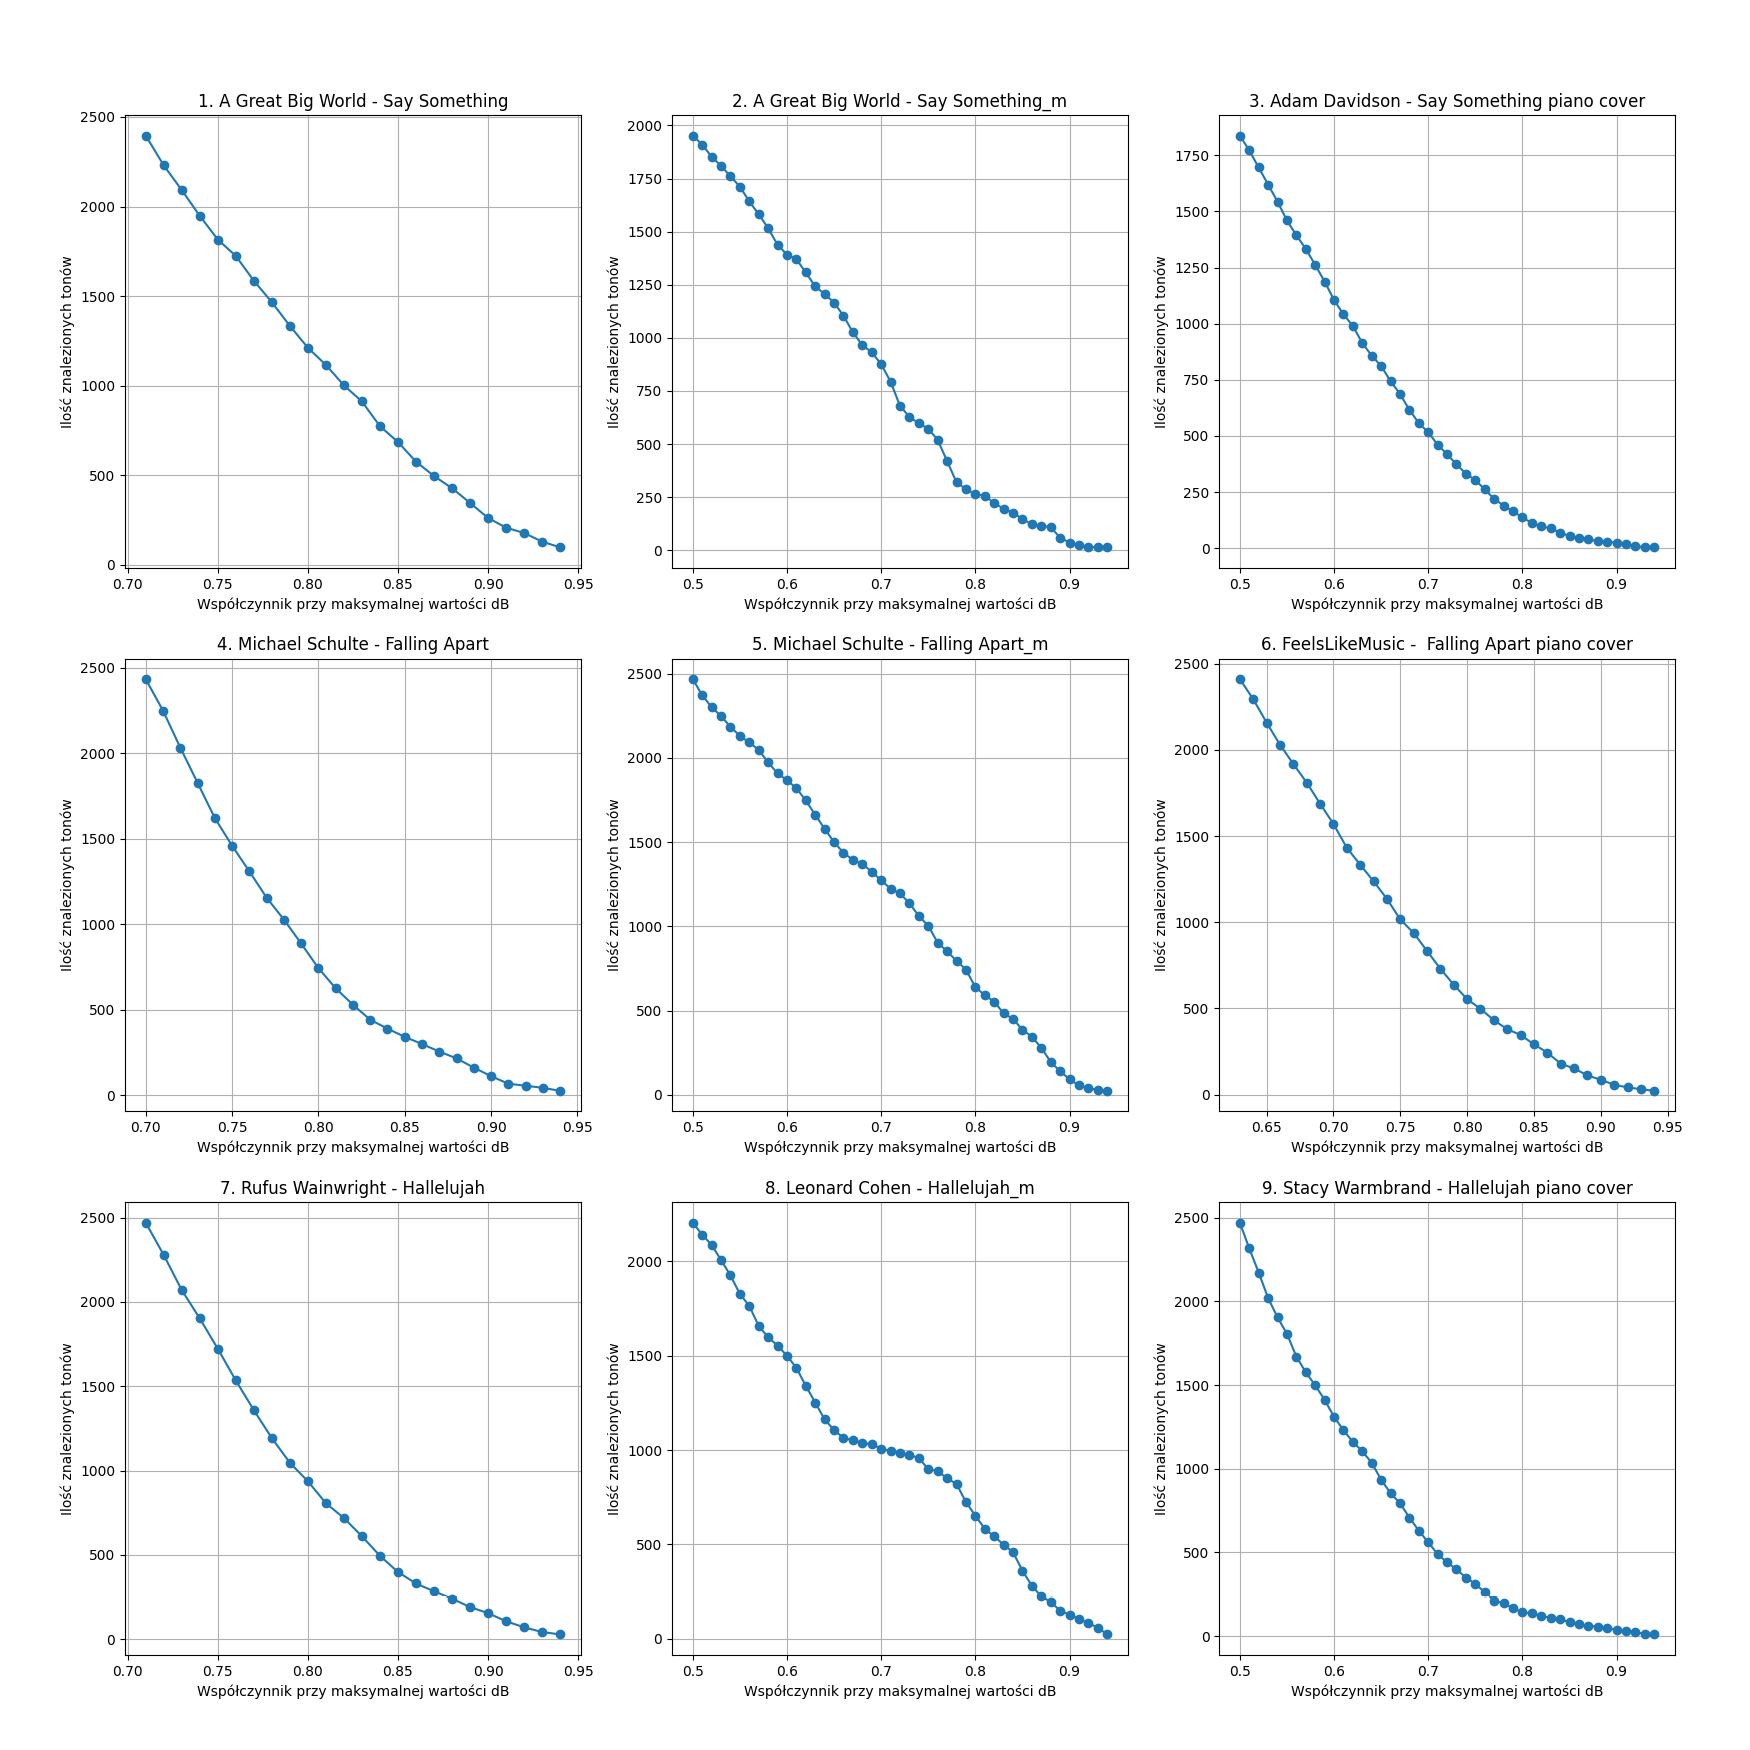
\includegraphics[width=0.94\textwidth]{img/5/wyk1.png}
  \caption{Wykres przedstawiający ilość wykrywanych tonów w metodzie pierwszej względem parametru m}
\end{figure}

Użycie tej metody dało bardzo dobre efekty przy utworze muzycznym stworzonym syntetycznie. Wykrywał składowe harmoniczne zrównujące się, bądź przewyższające amplitudę głównych dźwięków. Wyjściowa sekwencja z jednorazowo pomijanymi głównymi tonami oraz dodanymi przy błędnej identyfikacji dźwięków harmonicznych brzmiała identycznie jak wejściowa ścieżka audio. 

Przy utworze zagranym na pianinie nastąpił podział ze względu na zróżnicowanie amplitudowe wszystkich dźwięków. W bardziej wyciszonych fragmentach utworu metoda ta wykrywała pojedyncze dźwięki, bądź żadnych, natomiast we wzmocnionych momentach algorytm wykrywał zbyt wiele tonów wyłapując dźwięki harmoniczne oraz większe szumy, gdzie wyjściowa ścieżka dźwiękowa brzmiała podobnie do wejściowego utworu, jednakże przykryty wieloma źle zidentyfikowanymi dźwiękami. Jednakże fragmentami, gdzie każdy klawisz był grany z względnie równomierną siłą ścieżka wyjściowa brzmiała bardzo podobnie do piosenki poddanej analizie.
Przy analizie oryginalnego utworu, nastąpiły podobne problemy jak w analizie utworu granego na pianinie, jednakże dodatkowo powstały błędy w poprawności detekcji tonów w miejscach, gdzie przeplatały się dźwięki pianina oraz wokalu przez co powstawały dodatkowe luki w wynikowej sekwencji.

\subsection{Druga metoda detekcji głównych składowych utworu}

Metoda polegająca na wyznaczeniu progu granicznego z użyciem średniej ze wszystkich częstotliwości w małym przedziale czasu oraz maksymalnej wartości amplitudy. Współczynnik k oznaczał wartość, przez którą jest mnożona średnia oraz wchodził w skład wartości 1-k, przez którą mnożona jest maksymalna amplituda. Składowe następnie są sumowane i dzielone przez współczynnik d. Metoda ta jest wymaga przetwarzania znacznie więcej danych przez co jest zauważalnie wolniejsza niż pierwsza metoda.

W syntetycznych piosenkach metoda ta dała bardzo dobre efekty, ścieżka wyjściowa brzmiała również identycznie do wejściowej z pojedynczymi odchyłami, które lekko różniły się od poprzedniej metody w zależności od charakterystyki analizowanej piosenki.

Analiza gry na pianinie została poprawiona. Różnica pomiędzy fragmentami ścieżki audio została pomniejszona i detekcja stała się bardziej zbliżona do detekcji syntezowanej ścieżki dźwiękowej, niemniej jednak różnica nadal była widoczna.

Problem przy przetwarzaniu oryginalnego utworu pozostał nadal, pomimo poprawienia detekcji ogólnej. W konkretnych miejscach niejednokrotnie wykryte pianino zakrywało wokal, bądź odwrotnie w zależności od charakterystyki utworu.\\\\\\

\begin{figure}[h]
  \centering
  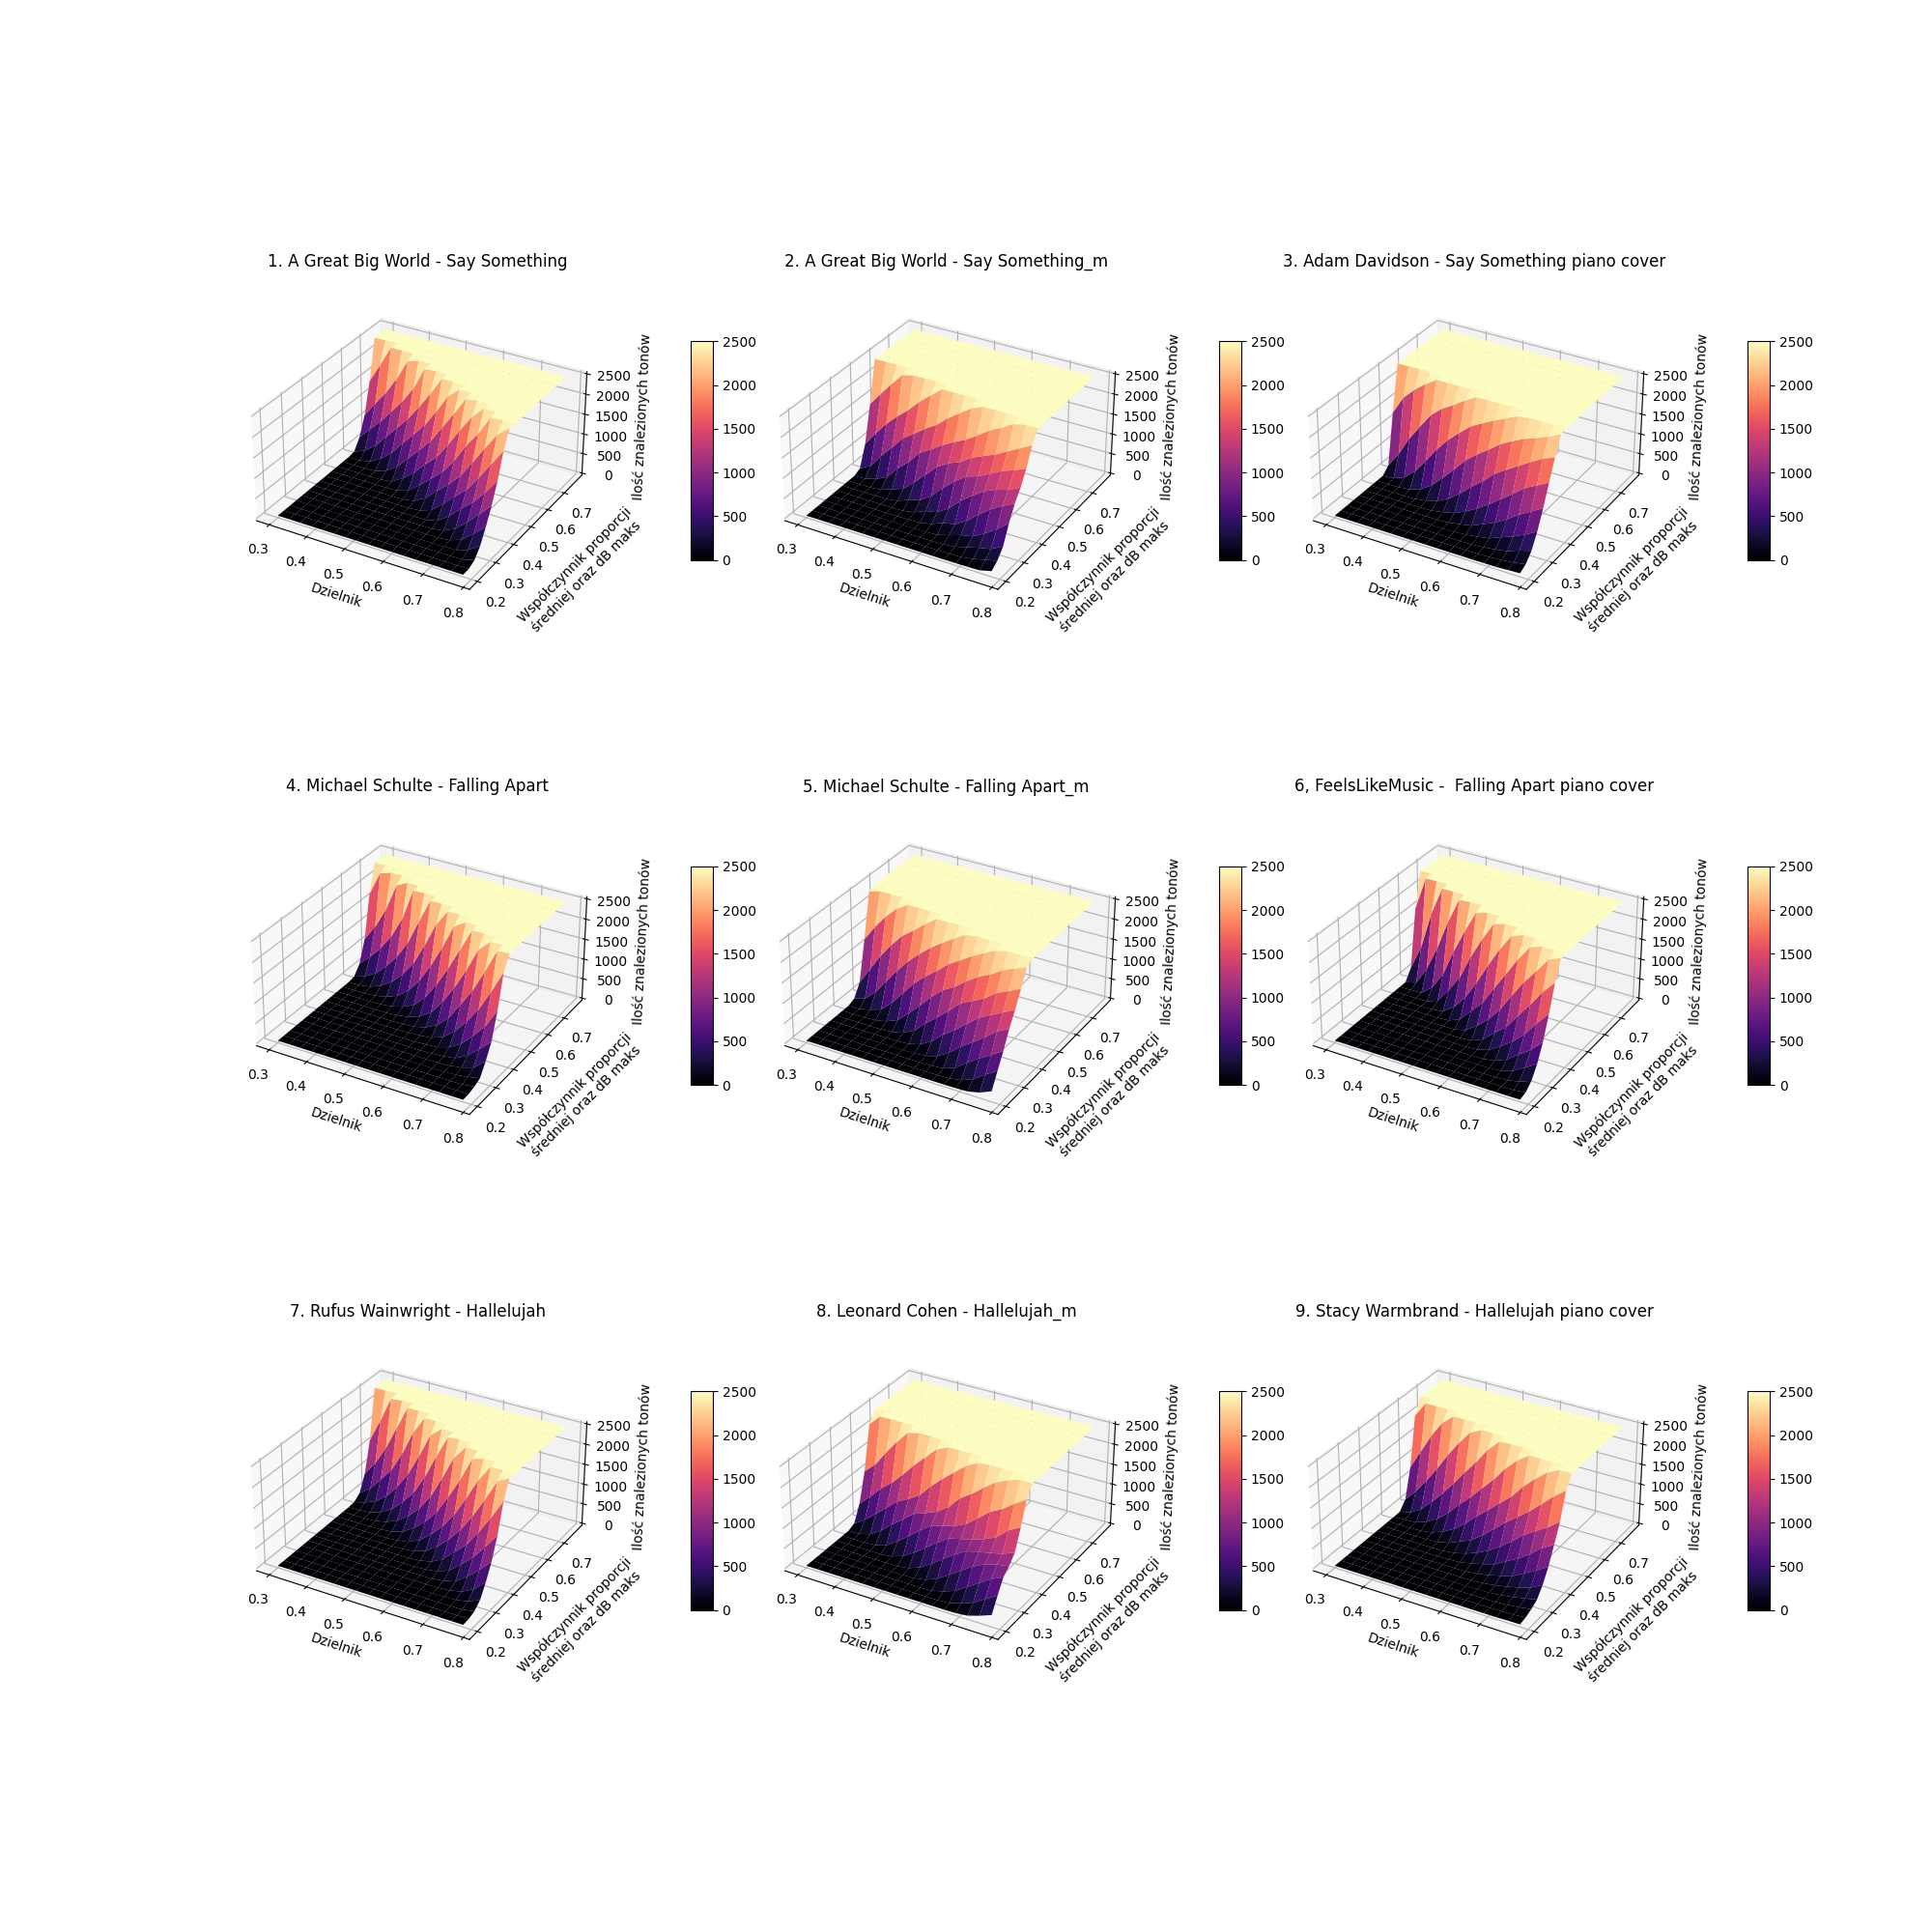
\includegraphics[width=0.94\textwidth]{img/5/wyk2.png}
  \caption{Wykres przedstawiający ilość wykrywanych tonów w metodzie drugiej względem parametrów k i d}
\end{figure}

\subsection{Trzecia metoda detekcji głównych składowych utworu}

Metoda polegająca na wyznaczeniu progu granicznego z użyciem maksymalnej wartości amplitudy oraz średniej ze wszystkich częstotliwości w małym przedziale czasu i małym przedziale częstotliwości. Współczynnik k oznaczał wartość, przez którą jest mnożona średnia oraz wchodził w skład wartości 1-k, przez którą mnożona jest maksymalna amplituda. Składowe następnie są sumowane i dzielone przez współczynnik d.

W syntetycznych piosenkach metoda ta dała również dobre efekty, jednakże identyfikując błędnie więcej składowych harmonicznych.\\

Analiza gry na pianinie została poprawiona. Różnica pomiędzy fragmentami ścieżki audio została jeszcze bardziej pomniejszona, jednak również wyłapując błędnie zauważalnie więcej składowych harmonicznych. Przetwarzanie oryginalnego utworu zostało nieznacznie poprawione, niestety kosztem uchwycenia niepożądanych częstotliwości.

\begin{figure}[h]
  \centering
  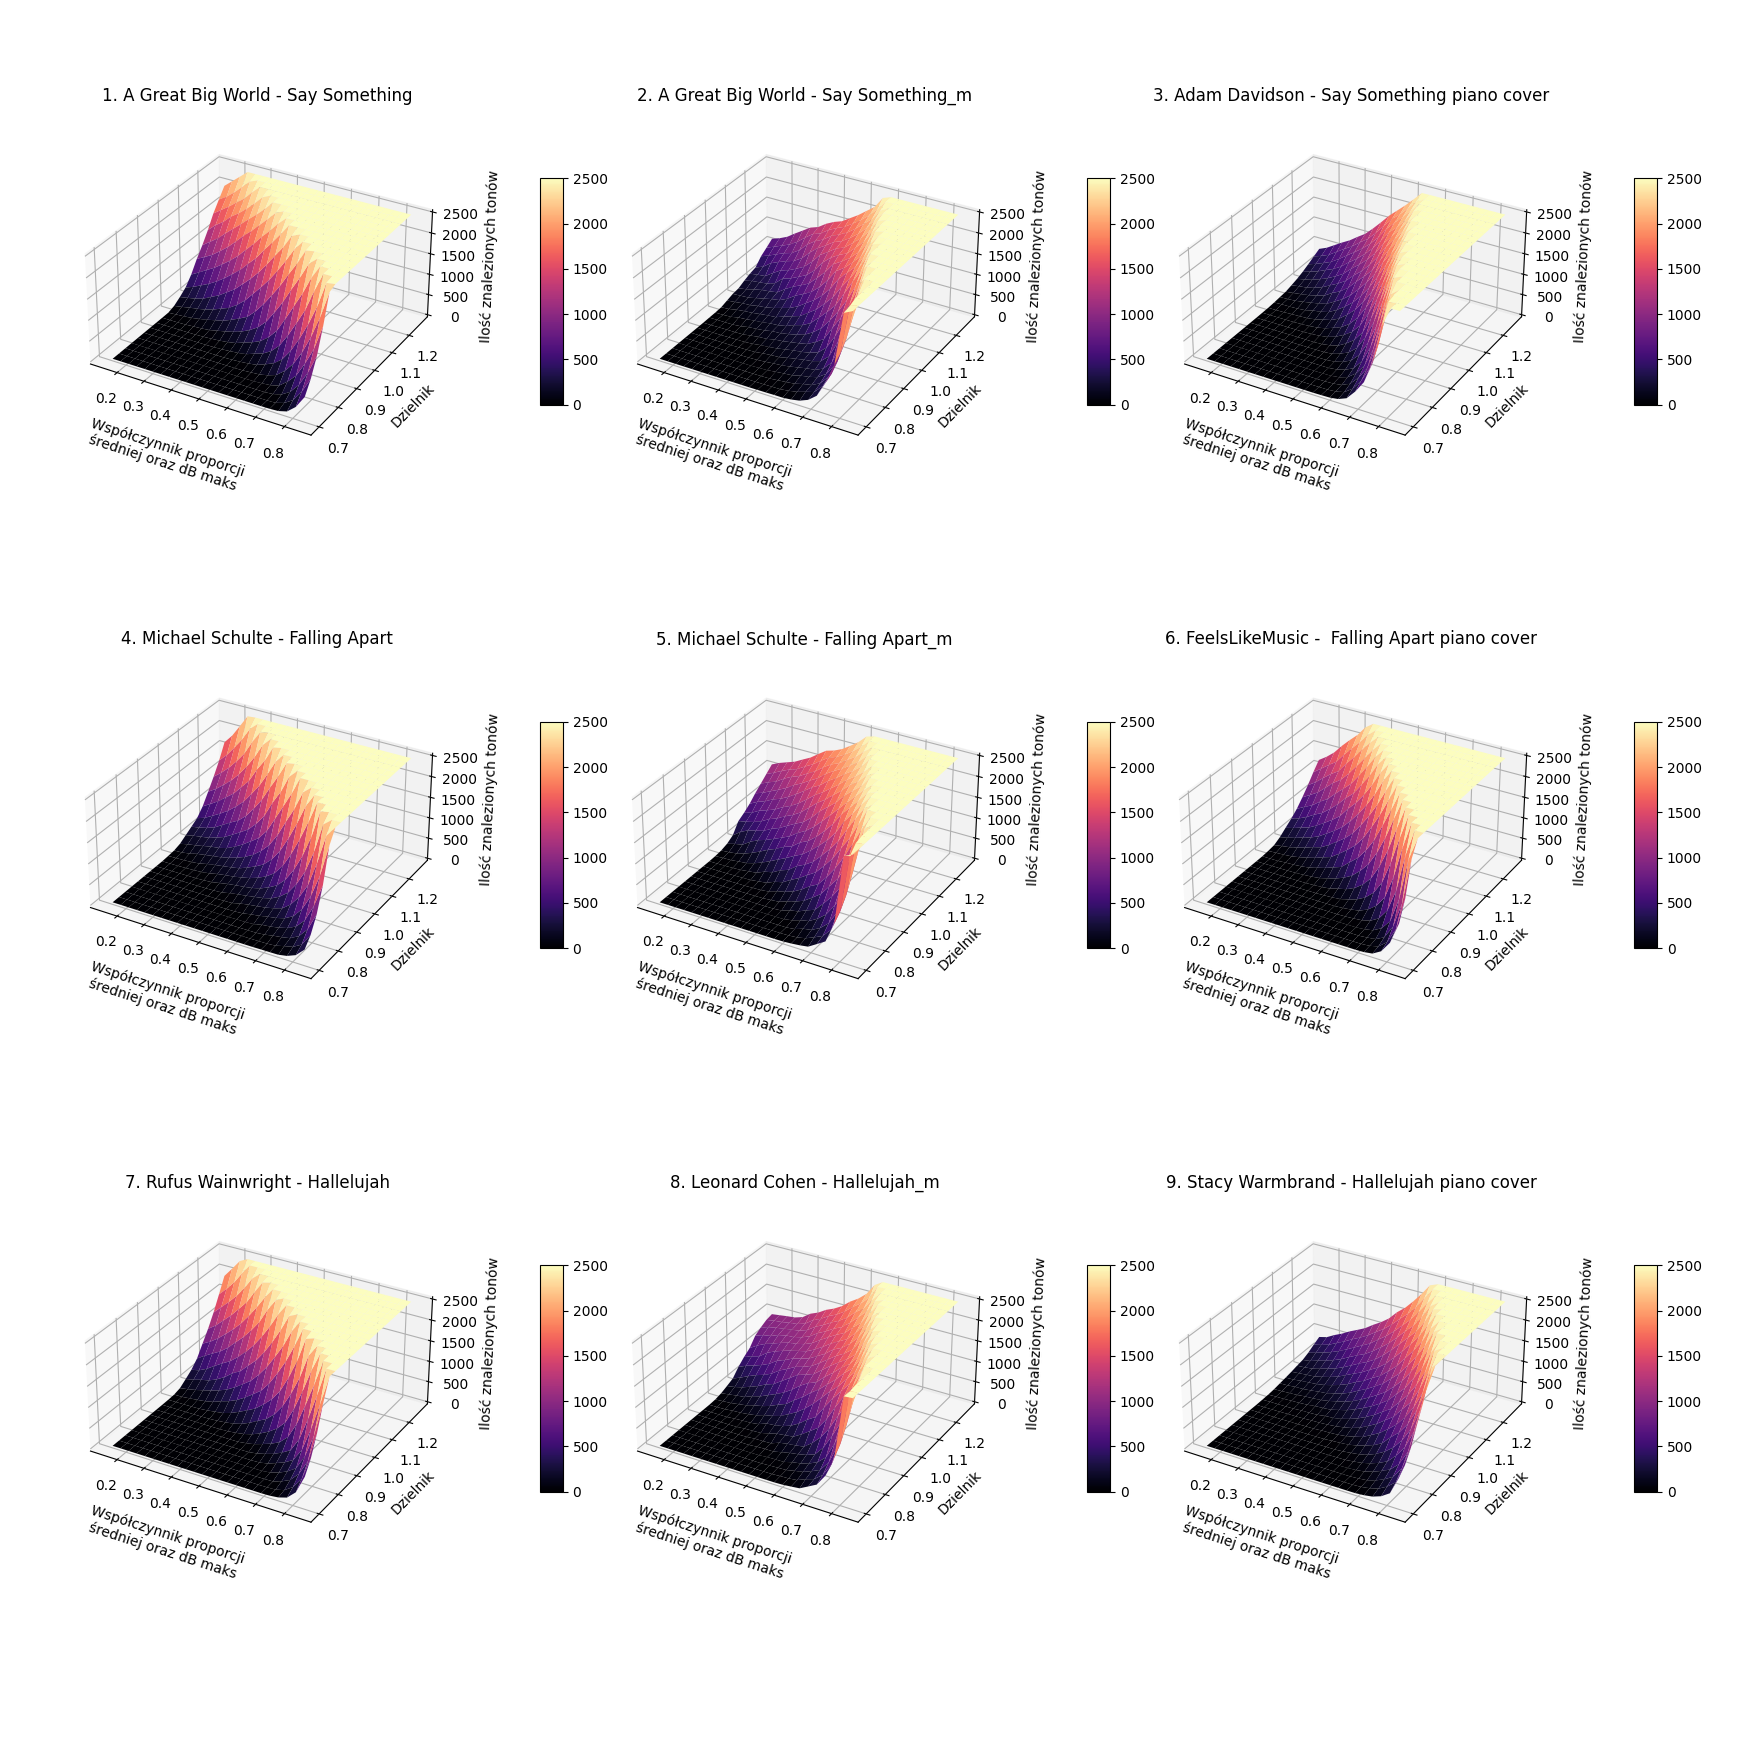
\includegraphics[width=0.94\textwidth]{img/5/wyk3.png}
  \caption{Wykres przedstawiający ilość wykrywanych tonów w metodzie trzeciej względem parametrów k i d}
\end{figure}

\newpage
\subsection{Say Something}

\textbf{Piosenka powstała z syntezy pliku midi}

\begin{figure}[h]
  \centering
  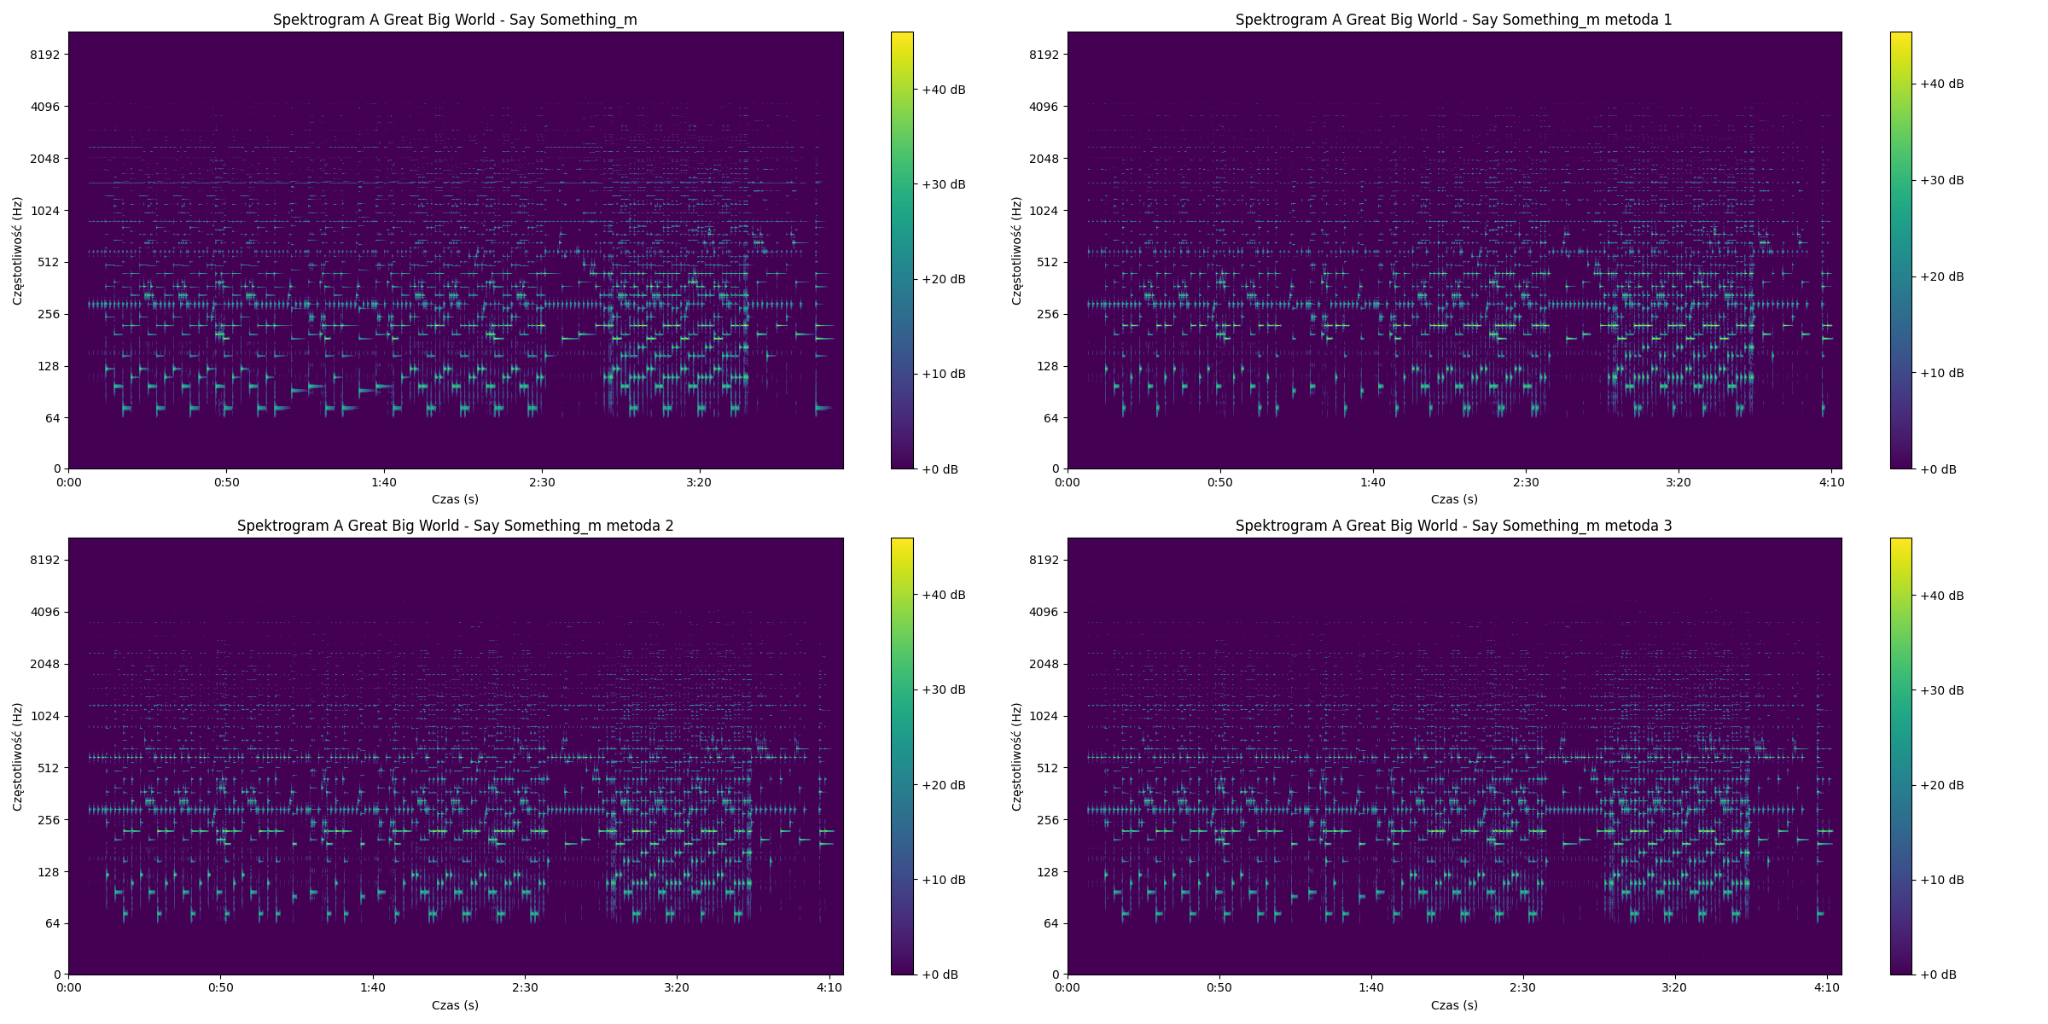
\includegraphics[width=0.82\textwidth]{img/5/wid1.png}
  \caption{Wykres przedstawiający widmo wejściowego nagrania oraz \\wyjściowych ścieżek dźwiękowych}
\end{figure}

\noindent Współczynnik m przy wartości maksymalnej użyty w pierwszej metodzie wynosił 0.66.
W drugiej metodzie współczynnik k, czyli stosunku średniej wszystkich wartości w małym otoczeniu czasu do wartości maksymalnej wynosił 0.4, a dzielnik d wynosił 0.6.
W trzeciej metodzie współczynnik k, czyli stosunku średniej wartości w małym otoczeniu do wartości maksymalnej wynosił 0.4, a dzielnik d wynosił 1.2.\\

\textbf{Piosenka zagrana na instrumencie klawiszowym typu pianino, bądź fortepian}

\begin{figure}[h]
  \centering
  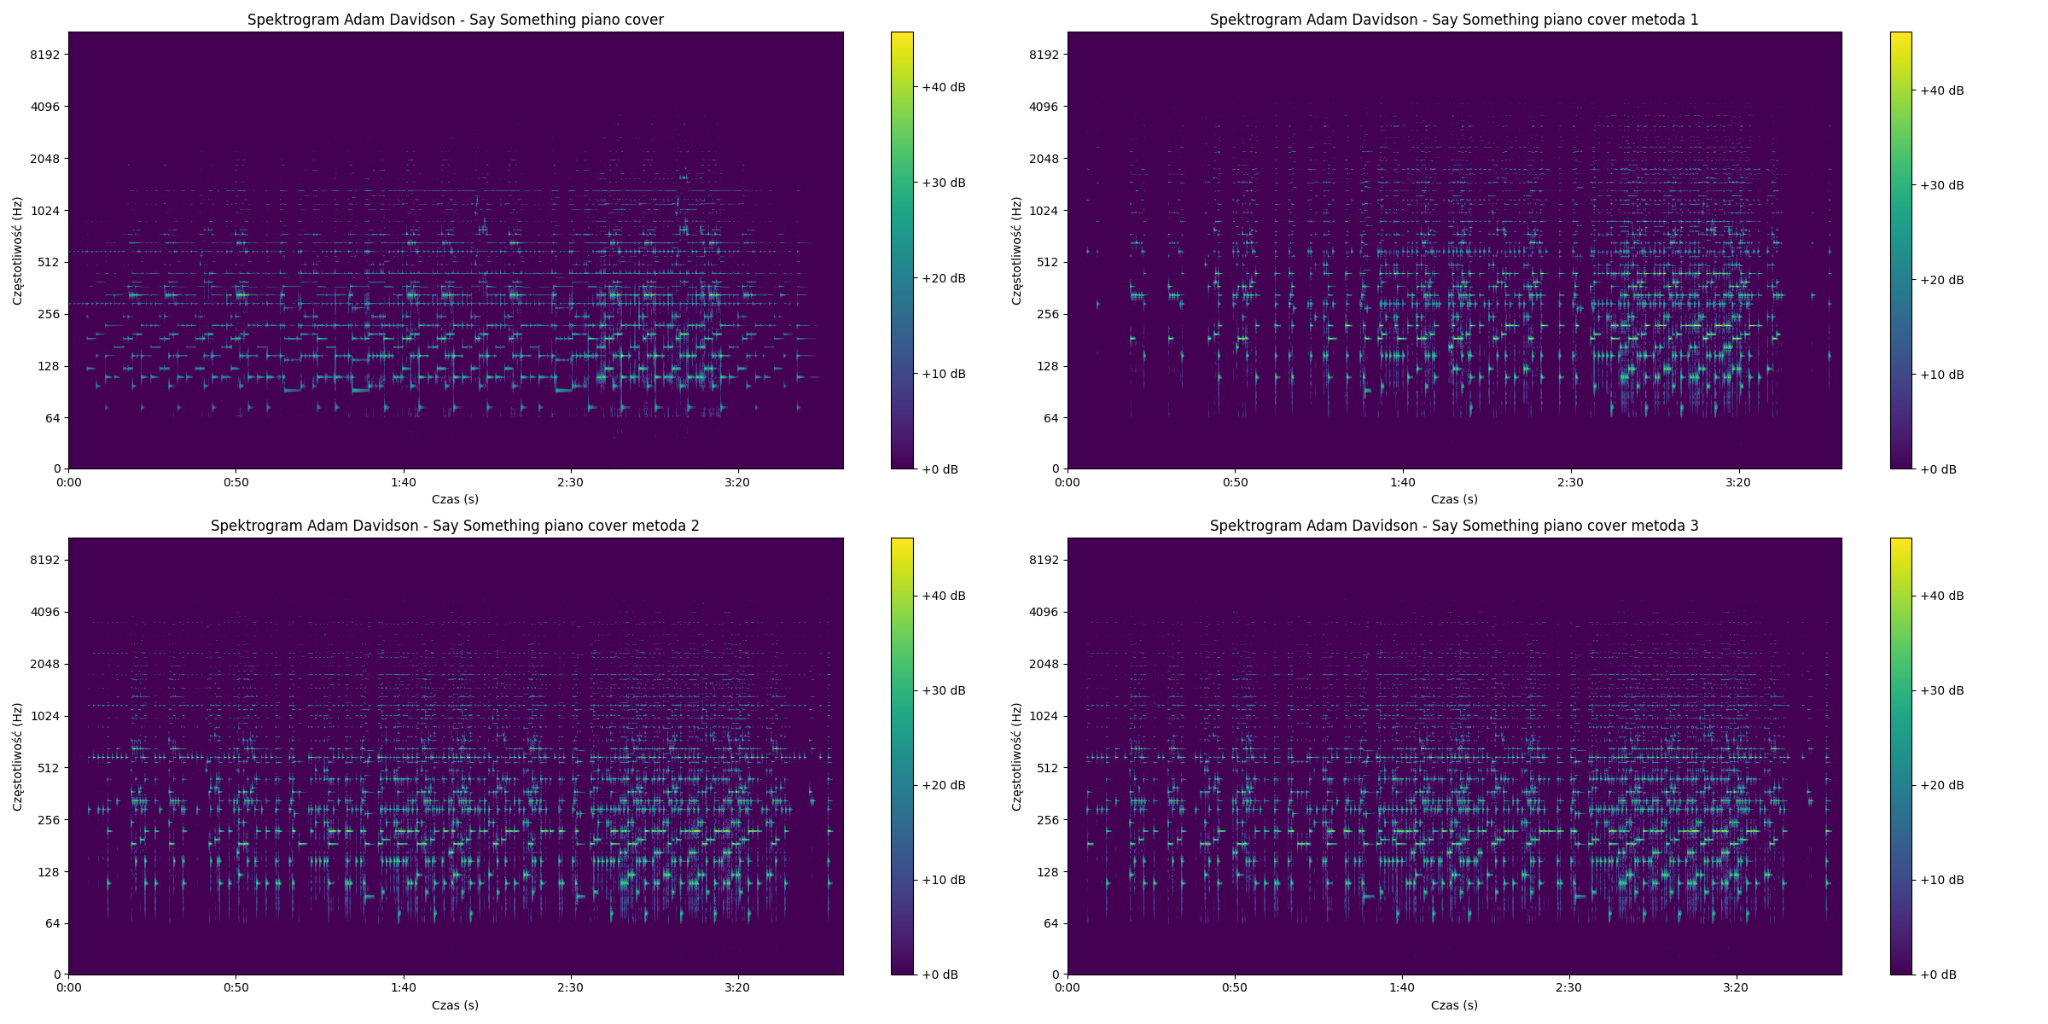
\includegraphics[width=0.82\textwidth]{img/5/wid2.png}
  \caption{Wykres przedstawiający widmo wejściowego nagrania oraz \\wyjściowych ścieżek dźwiękowych}
\end{figure}


\noindent Współczynnik m przy wartości maksymalnej użyty w pierwszej metodzie wynosił 0.62.
W drugiej metodzie współczynnik k, czyli stosunku średniej wszystkich wartości w małym otoczeniu czasu do wartości maksymalnej wynosił 0.4, a dzielnik d wynosił 0.6.
W trzeciej metodzie współczynnik k, czyli stosunku średniej wartości w małym otoczeniu do wartości maksymalnej wynosił 0.6, a dzielnik d wynosił 1.\\

\textbf{Oryginalna piosenka zawierająca wokal}

\begin{figure}[h]
  \centering
  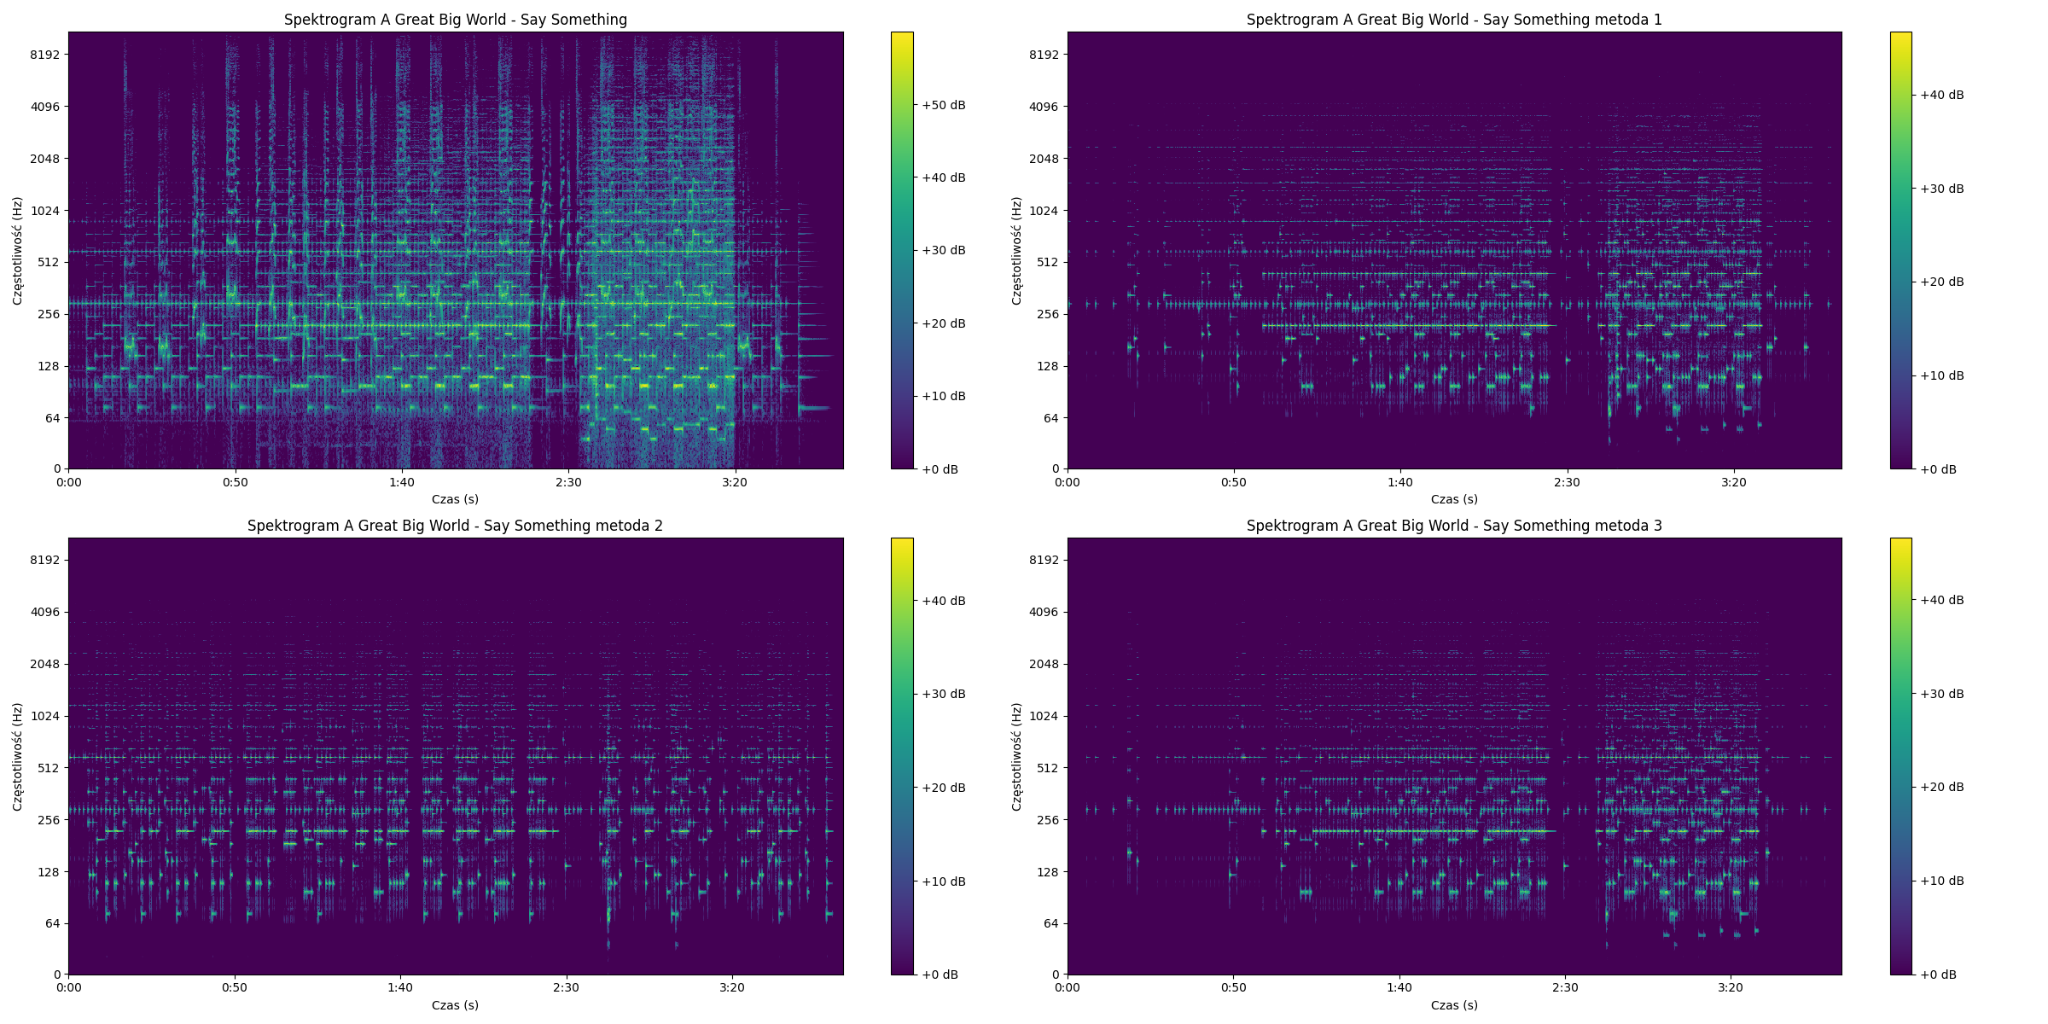
\includegraphics[width=0.82\textwidth]{img/5/wid3.png}
  \caption{Wykres przedstawiający widmo wejściowego nagrania oraz \\wyjściowych ścieżek dźwiękowych}
\end{figure}

\noindent Współczynnik m przy wartości maksymalnej użyty w pierwszej metodzie wynosił 0.76.
W drugiej metodzie współczynnik k, czyli czyli stosunku średniej wszystkich wartości w małym otoczeniu czasu do wartości maksymalnej wynosił 0.5, a dzielnik d wynosił 0.6.
W trzeciej metodzie współczynnik k, czyli stosunku średniej wartości w małym otoczeniu do wartości maksymalnej wynosił 0.3, a dzielnik d wynosił 1.1.

\newpage
\subsection{Hallelujah}

\textbf{Piosenka powstała z syntezy pliku midi}

\begin{figure}[h]
  \centering
  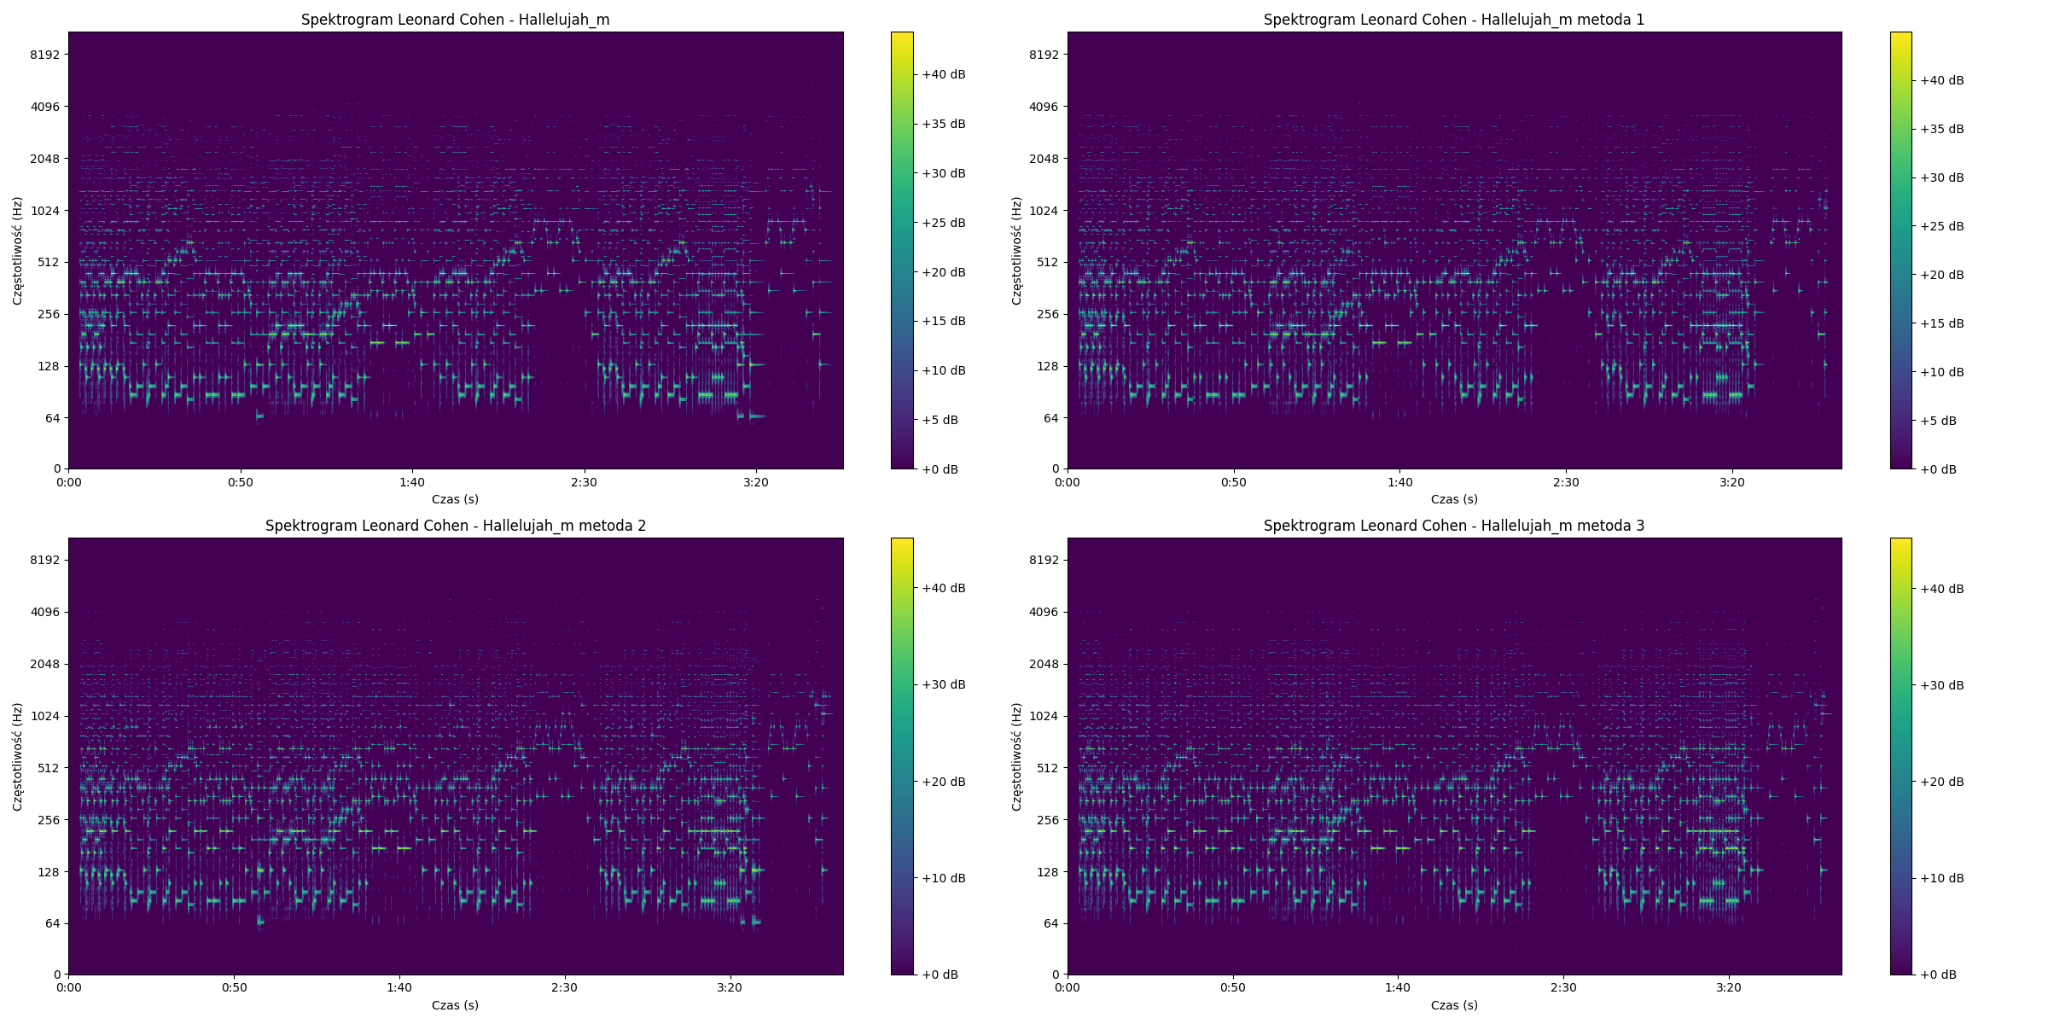
\includegraphics[width=0.82\textwidth]{img/5/wid4.png}
  \caption{Wykres przedstawiający widmo wejściowego nagrania oraz \\wyjściowych ścieżek dźwiękowych}
\end{figure}

\noindent Współczynnik m przy wartości maksymalnej użyty w pierwszej metodzie wynosił 0.66.
W drugiej metodzie współczynnik k, czyli stosunku średniej wszystkich wartości w małym otoczeniu czasu do wartości maksymalnej wynosił 0.4, a dzielnik d wynosił 0.6.
W trzeciej metodzie współczynnik k, czyli stosunku średniej wartości w małym otoczeniu do wartości maksymalnej wynosił 0.4, a dzielnik d wynosił 1.2.\\

\textbf{Piosenka zagrana na instrumencie klawiszowym typu pianino, bądź fortepian}

\begin{figure}[h]
  \centering
  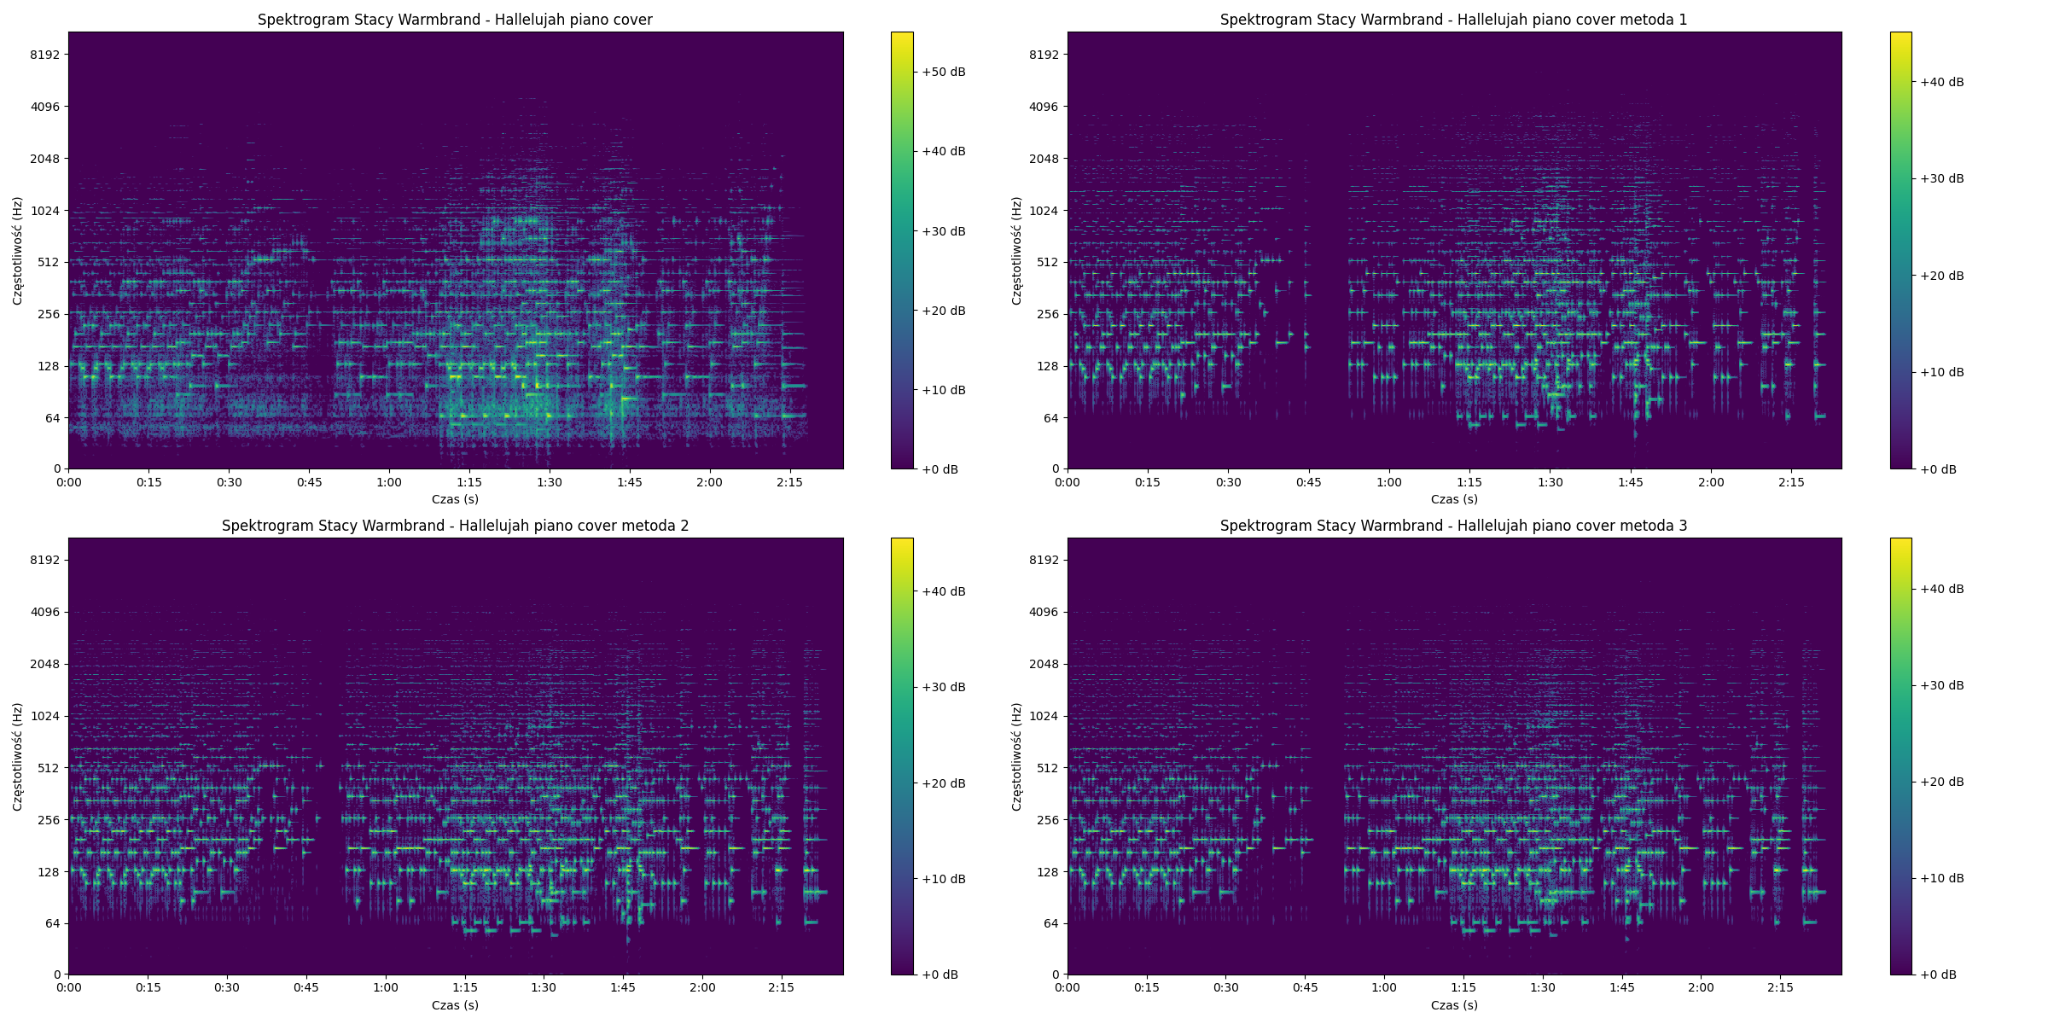
\includegraphics[width=0.82\textwidth]{img/5/wid5.png}
  \caption{Wykres przedstawiający widmo wejściowego nagrania oraz \\wyjściowych ścieżek dźwiękowych}
\end{figure}

\noindent Współczynnik m przy wartości maksymalnej użyty w pierwszej metodzie wynosił 0.64.
W drugiej metodzie współczynnik k, czyli stosunku średniej wszystkich wartości w małym otoczeniu czasu do wartości maksymalnej wynosił 0.5, a dzielnik d wynosił 0.55.
W trzeciej metodzie współczynnik k, czyli stosunku średniej wartości w małym otoczeniu do wartości maksymalnej wynosił 0.45, a dzielnik d wynosił 1.2.\\

\textbf{Oryginalna piosenka zawierająca wokal}

\begin{figure}[h]
  \centering
  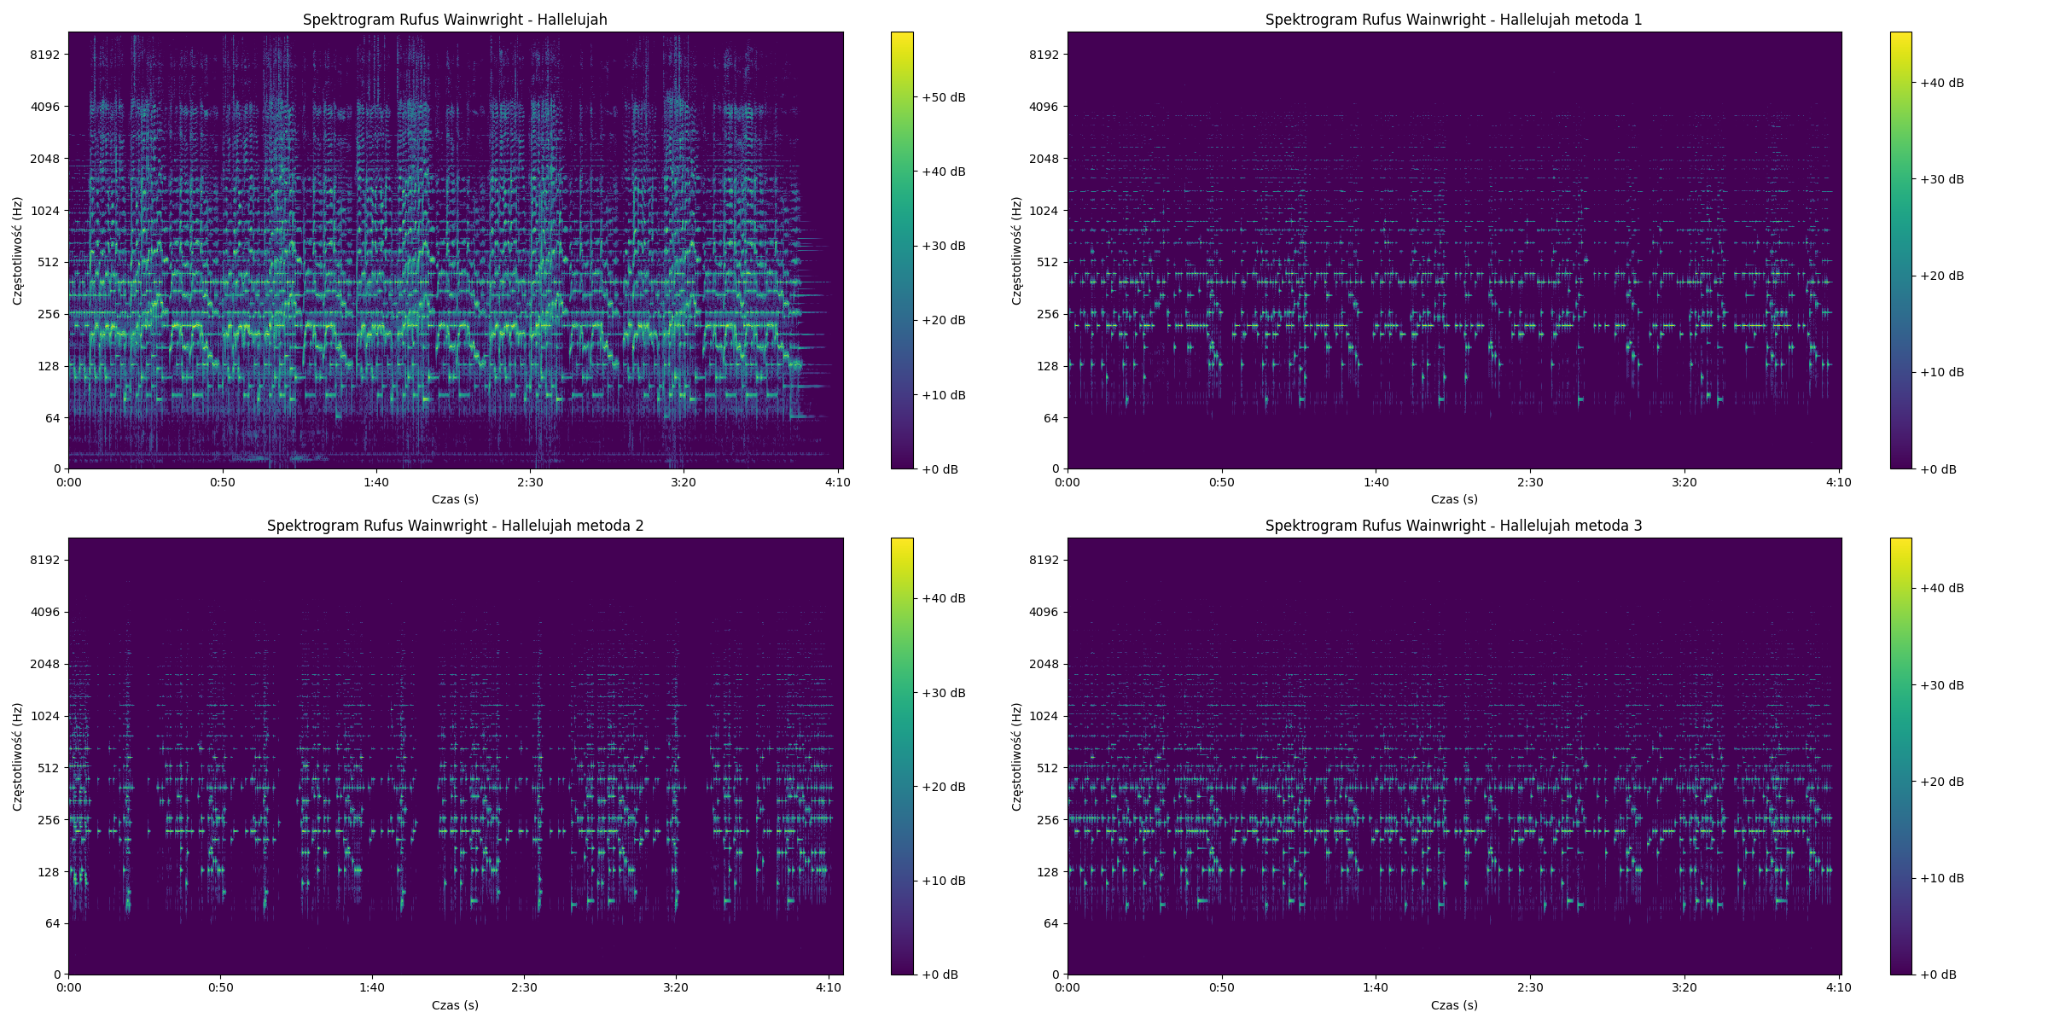
\includegraphics[width=0.82\textwidth]{img/5/wid6.png}
  \caption{Wykres przedstawiający widmo wejściowego nagrania oraz \\wyjściowych ścieżek dźwiękowych}
\end{figure}


\noindent Współczynnik m przy wartości maksymalnej użyty w pierwszej metodzie wynosił 0.79.
W drugiej metodzie współczynnik k, czyli stosunku średniej wszystkich wartości w małym otoczeniu czasu do wartości maksymalnej wynosił 0.6, a dzielnik d wynosił 0.46.
W trzeciej metodzie współczynnik k, czyli stosunku średniej wartości w małym otoczeniu do wartości maksymalnej wynosił 0.3, a dzielnik d wynosił 1.15.

\newpage
\subsection{Falling Apart}

\textbf{Piosenka powstała z syntezy pliku midi}

\begin{figure}[h]
  \centering
  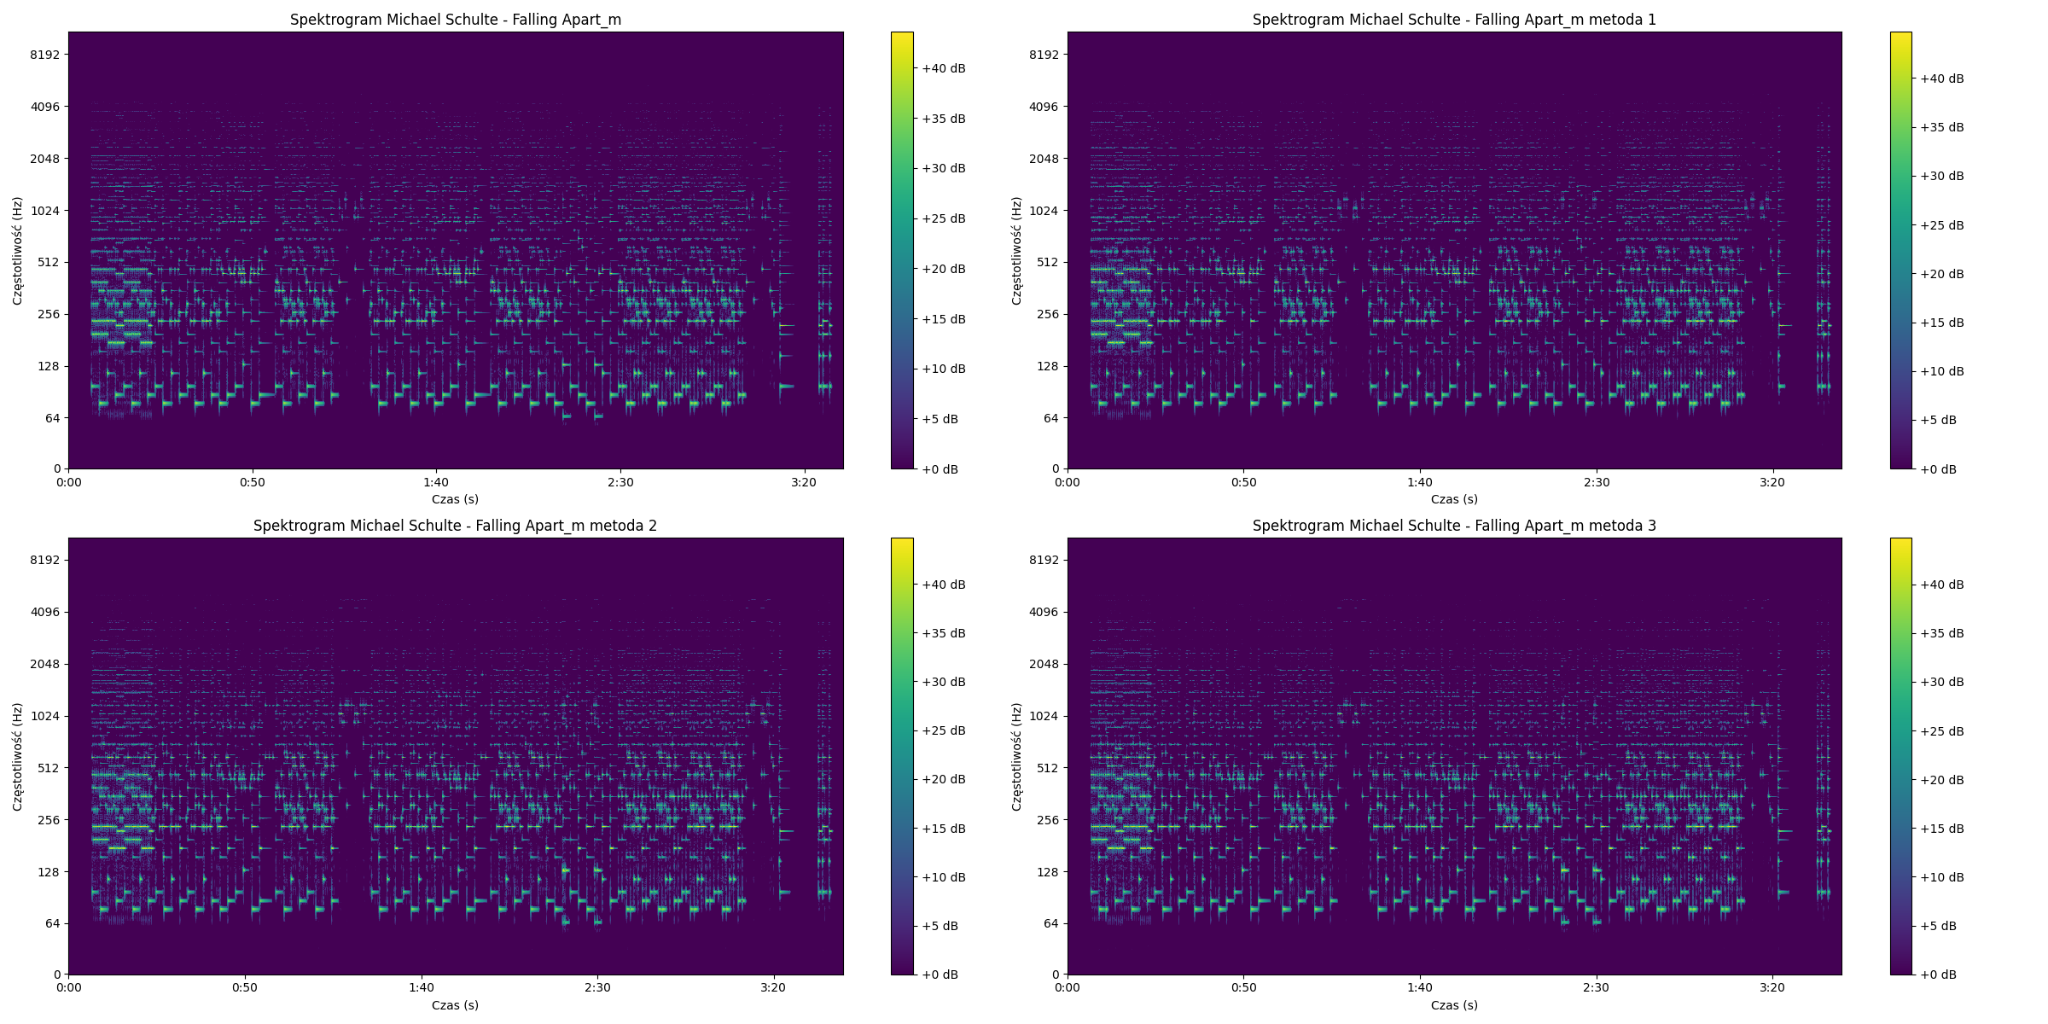
\includegraphics[width=0.82\textwidth]{img/5/wid7.png}
  \caption{Wykres przedstawiający widmo wejściowego nagrania oraz \\wyjściowych ścieżek dźwiękowych}
\end{figure}

\noindent Współczynnik m przy wartości maksymalnej użyty w pierwszej metodzie wynosił 0.66.
W drugiej metodzie współczynnik k, czyli stosunku średniej wszystkich wartości w małym otoczeniu czasu do wartości maksymalnej wynosił 0.4, a dzielnik d wynosił 0.6.
W trzeciej metodzie współczynnik k, czyli stosunku średniej wartości w małym otoczeniu do wartości maksymalnej wynosił 0.4, a dzielnik d wynosił 1.2.\\

\textbf{Piosenka zagrana na instrumencie klawiszowym typu pianino, bądź fortepian}

\begin{figure}[h]
  \centering
  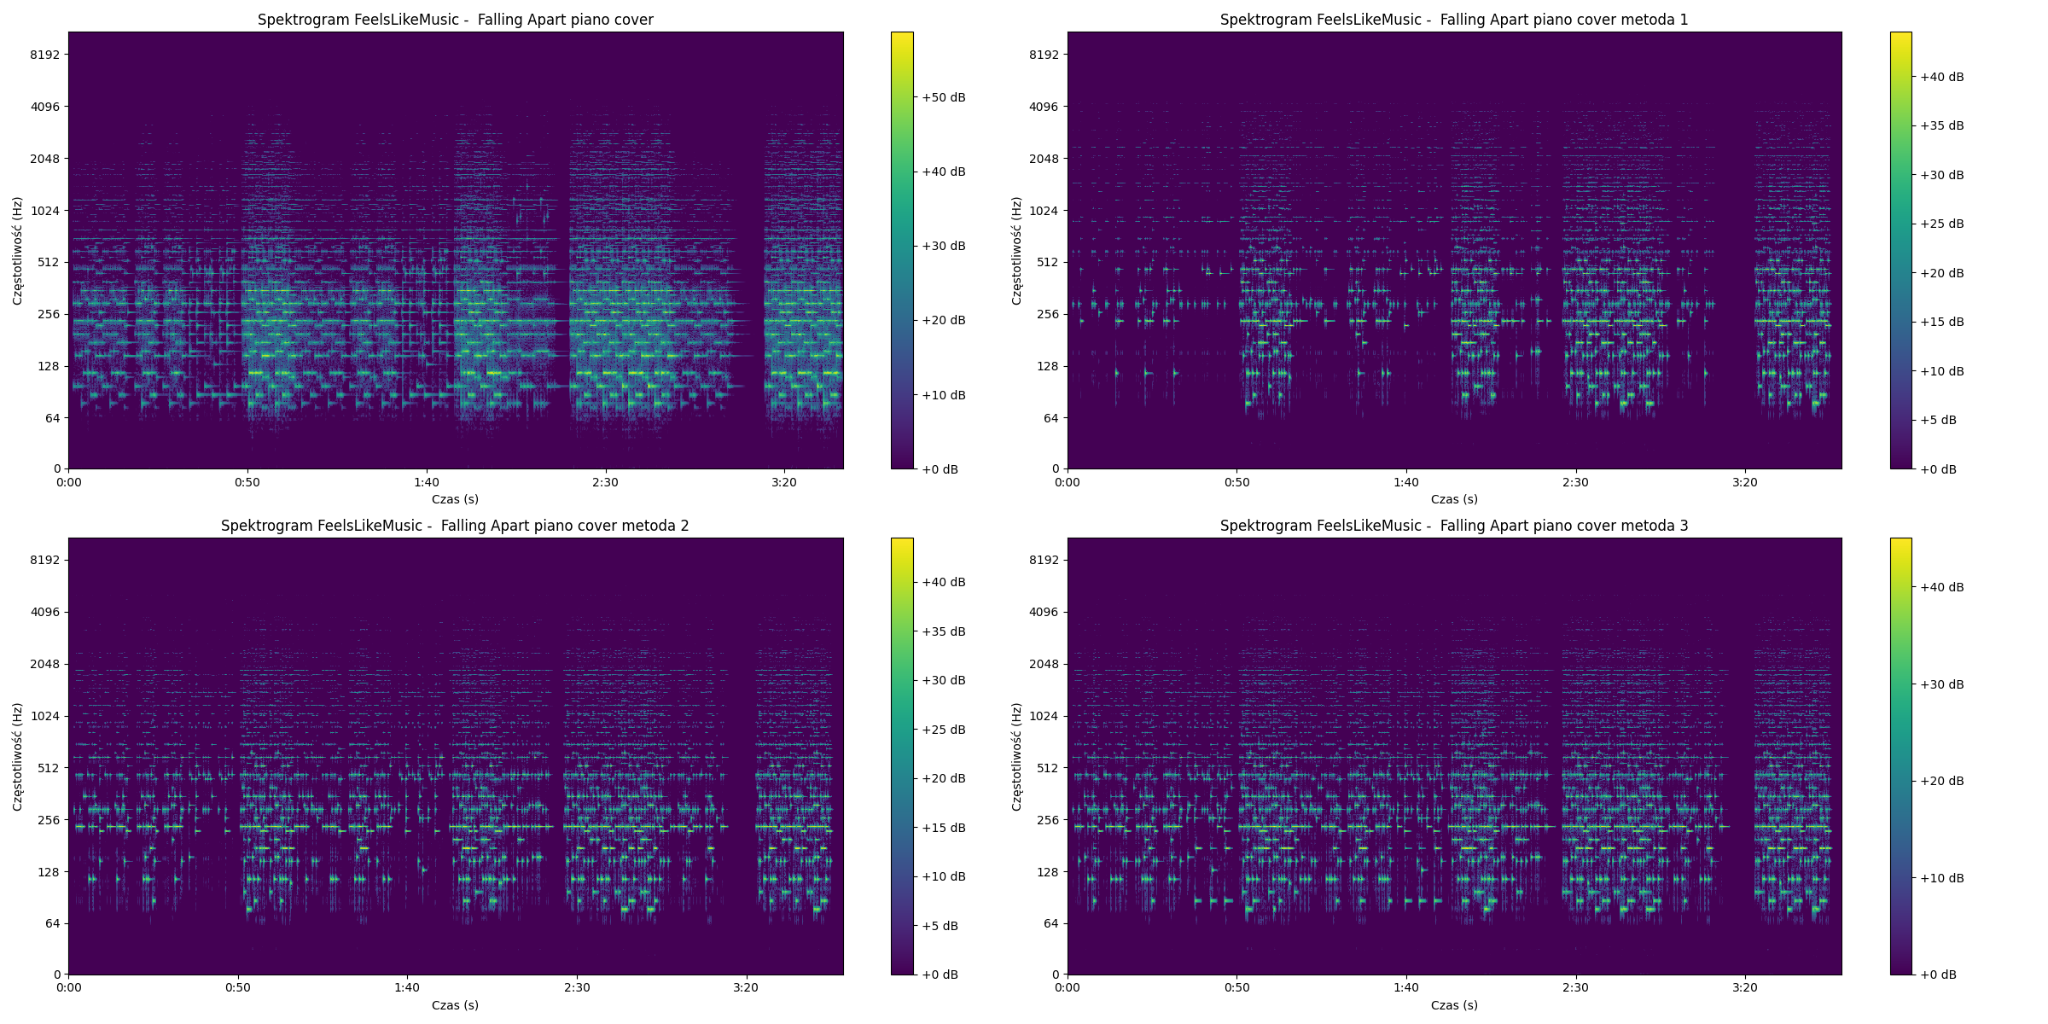
\includegraphics[width=0.82\textwidth]{img/5/wid8.png}
  \caption{Wykres przedstawiający widmo wejściowego nagrania oraz \\wyjściowych ścieżek dźwiękowych}
\end{figure}

\noindent Współczynnik m przy wartości maksymalnej użyty w pierwszej metodzie wynosił 0.71.
W drugiej metodzie współczynnik k, czyli stosunku średniej wszystkich wartości w małym otoczeniu czasu do wartości maksymalnej wynosił 0.5, a dzielnik d wynosił 0.53.
W trzeciej metodzie współczynnik k, czyli stosunku średniej wartości w małym otoczeniu do wartości maksymalnej wynosił 0.5, a dzielnik d wynosił 1.1.\\

\textbf{Oryginalna piosenka zawierająca wokal}


\begin{figure}[h]
  \centering
  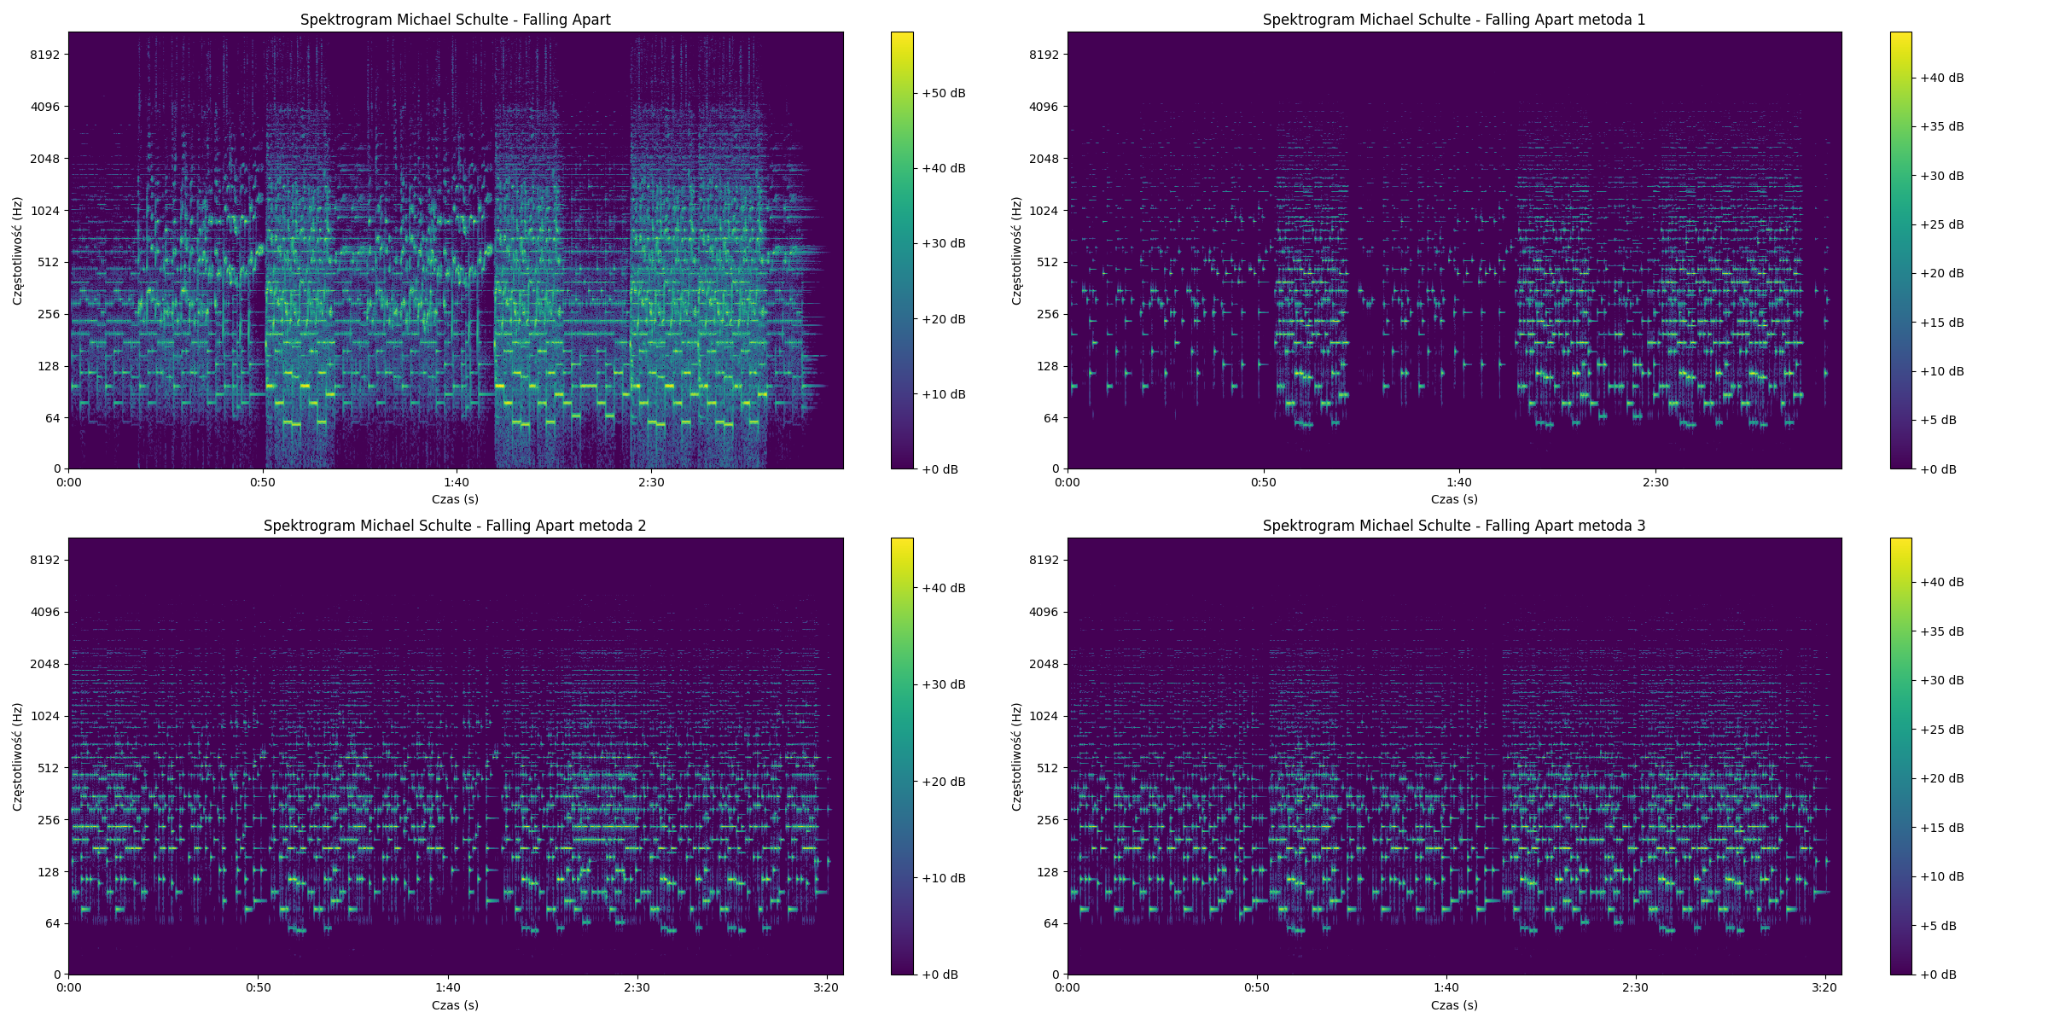
\includegraphics[width=0.82\textwidth]{img/5/wid9.png}
  \caption{Wykres przedstawiający widmo wejściowego nagrania oraz \\wyjściowych ścieżek dźwiękowych}
\end{figure}

\noindent Współczynnik m przy wartości maksymalnej użyty w pierwszej metodzie wynosił 0.75.
W drugiej metodzie współczynnik k, czyli stosunku średniej wszystkich wartości w małym otoczeniu czasu do wartości maksymalnej wynosił 0.6, a dzielnik d wynosił 0.46.
W trzeciej metodzie współczynnik k, czyli stosunku średniej wartości w małym otoczeniu do wartości maksymalnej wynosił 0.6, a dzielnik d wynosił 1.

\subsection{Wyświetlanie synthesii}

Wszystkie wskazówki graficzne są poprawnie wyświetlane ze względu na ton. We fragmentach, w których naciskane jest więcej klawiszy w jednym momencie, program ze względu na swoją prędkość działania powoduje opóźnienie w pojawieniu się każdego klawisza, przez co powstaje niewielkie przesunięcie względem siebie. Natomiast ze względu na potrzebę użycia akumulatora, który kompensuje opóźnienia zależne od ilości wyświetlanych elementów, potrafi nie zgadzać się ich długość. Spowodowane jest to wpływem zmiennej prędkości wyświetlania na długość trwania każdego tonu.

\section{Analiza i ocena poprawności odtwarzania tonów}

Wyjściowa sekwencja muzyczna wybrzmiewała identycznie dla wejściowej syntetycznie wygenerowanej piosenki. Każda z metod świetnie się sprawuje przy tak stworzonym dźwięku. Powodem tego jest praktycznie stały poziom amplitudy dla wszystkich głównych dźwięków oraz dobra identyfikacja dźwięków harmonicznych, które zwykle rozpoczynają się równo z dźwiękiem, z którego powstały, dzięki czemu niewiele z nich wybrzmiewa w wynikowej sekwencji.

Utwór muzyczny grany na pianinie przyniósł znacznie słabszą jakość detekcji. Pierwsza metoda, gdzie parametr graniczny był stały nie radził sobie z amplitudą zmieniającą się wraz z każdym pojedynczym dźwiękiem. W ten sposób powstały miejsca wyciszenia, gdzie nie został żaden dźwięk wyłapany, bądź pojedyncze oraz miejsca zgłośnień, gdzie zmiana dynamiki gry na bardziej eksplozywną powodowała wyłapanie wielu składowych harmonicznych, które potrafiły kompletnie zniekształcić piosenkę. Dużo lepiej tutaj radziła sobie metoda druga, która zmieniała parametr detekcji wraz z czasem piosenki, przez co zmienna dynamika nie stanowiła już takiego problemu, jak przy użyciu poprzedniej metody. Jednakże wynik zauważalnie odbiega od wyniku przy syntezowanej piosence. Spowodowane jest to bogactwem i głębią dźwięku, co za tym idzie, złożeniem składowych harmonicznych, które bardzo utrudniają analizę utworu. Trzecia metoda, radziła sobie podobnie do drugiej metody, momentami znajdując więcej poprawnych tonów, niemniej jednak kosztem przechwytywania większej ilości dźwięków harmonicznych. Powodem tego jest dobieranie progu ze względu na najbliższe otoczenie, co pomaga znaleźć wśród reszty tony o niższej amplitudzie, jak i zarazem składowe harmoniczne, które nie 
odznaczały się tak bardzo głośnością, aby zostać wykryte przez poprzednie algorytmy.

Analiza oryginalnego utworu muzycznego przyniosła podobne efekty co utworu granego na pianinie z mniejszą dokładnością. Pierwsza metoda nie poradziła sobie ze zmiennością amplitudy w czasie, co przełożyło się na miejsca z widocznymi dziurami oraz miejsca przesilenia ilości wykrytych tonów. Druga metoda radziła sobie gorzej niż w poprzednim typie utworu muzycznego. Zmienność progu detekcji zależnej od czasu, nie radził sobie ze zmiennością amplitudy pomiędzy wokalem a instrumentami, co powodowało częste luki w detekcji śpiewu. Trzecia metoda poradziła sobie z oryginalnym utworem podobnie do wersji odtworzonej na pianinie. Różnica w amplitudach wokalu i instrumentów nie była tak znacząca, dzięki zmienności progu detekcji w zależności od najbliższego otoczenia, co niestety wciąż przekłada się na wrażliwość tej metody na dźwięki harmoniczne o niższej amplitudzie, które nie były wykrywane przez pozostałe metody.

Detekcja czasu rozpoczęcia się danego dźwięku, w każdym scenariuszu testowym była na wysokim poziomie. Wyszukiwanie maksimum lokalnego i cofanie się do kolejnego punktu przegięcia pozwalało rozpocząć dźwięk równo z zauważeniem wzrostu amplitudy przez jego zagranie. Tylko w nielicznych momentach mogło zostać to zagłuszone przez główne tony lub dźwięki harmoniczne o bardzo bliskiej częstotliwości. Detekcja czasu trwania dźwięku jest poprawna, jednak mało dokładna. Powodem jest stały próg zakończenia trwania dźwięku. Nie mógł zostać zdefiniowany jako znalezienie minimum lokalnego, którym rzeczywiście charakteryzuje się zakończony dźwięk, ponieważ w czasie jego trwania, pozostałe tony, które odznaczają się składowymi harmonicznymi na podobnej częstotliwości, mogłyby powodować znacząco przedwczesne zakończenie się trwania tonu.

\section{Problemy i ograniczenia napotkane podczas implementacji}

Jednym z najtrudniejszych problemów okazała się zmienność amplitudy w piosence, co wymagało zaimplementowania bardziej skomplikowanych metod detekcji. Trudność ta spowodowała również niedokładność przy przeplataniu się dwóch instrumentów, bądź ich składowych harmonicznych, co powodowało brak wykrywalności wielu tonów, które zostawały przykryte przez silniejszy sygnał.
Barierą nie do pokonania w pełni okazały się składowe harmoniczne, które jak wcześniej zostało wspomniane niejednokrotnie odznaczały się jako główne dźwięki, których nie sposób jednoznacznie zidentyfikować.

        \chapter{Podsumowanie}
\vspace{-25pt}

\section{Osiągnięte cele}

Udało się stworzyć funkcjonalną grę zintegrowaną z elektronicznym instrumentem klawiszowym wyświetlającą synthesie z własnoręcznie wybranego pliku muzycznego, która realnie pozwala na naukę gry na instrumencie klawiszowym oraz na rywalizację polegającej na zdobyciu jak największej ilości punktów. Natomiast konwersja z formatu mp3 na format midi potrzebny do wyświetlenia synthesii piosenki powiodła się, niemniej jednak zbyt mało dokładnie, aby była funkcjonalna na tyle na ile zakładano na początku projektu.

\section{Wnioski}

Transformata Fouriera okazała się być niewystarczającym narzędziem, aby w pełni odtworzyć sekwencję muzyczną, z której powstał dany utwór. Jednakże jest narzędziem koniecznym przy przetwarzaniu sygnałów dźwiękowych, ponieważ większość dźwięków była poprawnie rozpoznawana oraz bardzo dokładne zostawał wyznaczany czas ich rozpoczęcia. 

\section{Możliwe korekty i ulepszenia}

Algorytm mógłby zostać poprawiony wraz z użyciem dodatkowych narzędzi takich jak uczenie maszynowe, mogłoby pomóc w klasyfikacji głównych dźwięków, z których składa się piosenka oraz składowych harmonicznych.
Natomiast wyświetlanie synthesii mogłoby zostać poprawione używajac języka kompilowanego zamiast interpretowanego, co pozwoliłoby na zoptymalizowanie działania funkcji wyświetlającej sekwencje muzyczną.

\section{Wskazanie dalszych kierunków rozwoju projektu}

Problem składowych harmonicznych oraz doboru progu wykrywania tonów mógłby zostać rozwiązany przy użyciu uczenia maszynowego. Ze względu na zróżnicowaną barwę dźwięku każdego instrumentu, byłaby możliwość podzielenia na każdy z osobna. Na podstawie plików midi i różnych metod syntezy dźwięku można wytrenować model, klasyfikujący dźwięk do odpowiedniego tonu. Następnie wykorzystać go do wcześniej podzielonych części audio posiadających jednolitą barwę, w celu rozpoznania początkowej sekwencji muzycznej.

Po uzyskaniu w pełni poprawnej detekcji projekt mógłby zostać uzupełniony o przetwarzanie na bieżąco gry użytkownika poprzez mikrofon zamiast bezpośredniego łącza i detekcję granych tonów. To otworzyłoby drzwi na możliwość stworzenia części z użyciem innego instrumentu niż klawiszowy.

Kolejnym krokiem byłoby dodanie różnych funkcjonalności do gry takie jak tryb nauki, w którym jest możliwość zatrzymania się w każdym momencie, możliwość zapisu własnej gry i porównanie do wzorcowej piosenki oraz zmiany kosmetyczne w celu odświeżenia szaty graficznej.

        
	\printbibliography

\end{document}

